
\subsubsection*{2.2 Personnel, Level of Effort, and Review Authority}
\textbf{Lu Sun, Principal Investigator,} holds a B.S. in Mathematics and an M.S. in Industrial and Systems Engineering. Her research and manufacturing experience supports uncertainty-aware decision modeling, benchmark design, evaluation, and integration of technical and operational constraints. She will devote approximately full-time to technical direction, Objectives 1 and 3, evaluation, research integration, and NSF reporting.

\textbf{Mengmeng Wang, Key Personnel,} brings electrical engineering, fault-detection, robotics, and physical-system validation experience. She will devote approximately full time to reference architecture, component/interface constraints, safety boundaries, physical testing, and engineering review. She will hold approval authority for the low-voltage reference designs and test procedures used in Phase I.

\textbf{Software/AI engineering personnel} will devote approximately 4.0 person-months to the evidence graph, document/image processing, constraint engine, model orchestration, evaluation tooling, secure data handling, and prototype interface. A \textbf{budgeted independent electrical-engineering reviewer} will contribute approximately 1.0 person-month to blinded benchmark annotation, inter-rater review, safety-case adjudication, and final technical audit. Interns or research assistants may support documentation and test execution but will not have independent design or safety approval authority.

\vspace{-3pt}
\begin{table}[H]
\centering
\small
\begin{tabularx}{\textwidth}{P{0.15\textwidth}P{0.10\textwidth}YP{0.16\textwidth}}
\toprule
% \rowcolor{darkteal}
% \textcolor{white}
{\textbf{Role}} &
% \textcolor{white}
{\textbf{Effort}} &
% \textcolor{white}
{\textbf{Primary Responsibility}} &
% \textcolor{white}
{\textbf{Authority}} \\
\midrule
PI (Lu Sun) & 12 PM & Uncertainty-aware decision methods, clarification policy, and test-plan integration & Final go/no-go review \\
\rowcolor{lighttablegray}
Key Personnel (\mbox{Mengmeng Wang}) & Full-Time & Reference designs, electrical and physical constraints, fault injection, and prototype validation & Reference design sign-off \\
Software/AI Team & 4.0 PM & Evidence graph, constraint engine, multimodal pipeline, and secure prototype interface & Reviewed by PI \\
\rowcolor{lighttablegray}
Independent Reviewer (EE) & 1.0 PM & Blinded benchmark annotation, inter-rater review, safety-case adjudication, and final audit & Independent audit \\
ACC Partners & In-Kind & Workflow context, user needs, and pilot planning input & No sign-off role \\
\toprule
\end{tabularx}
\caption{Phase I responsibility and review-authority matrix.}
\label{tab:team}
\end{table}
\vspace{-10pt}

The project will use standard secure software-development infrastructure and a low-voltage prototyping environment including regulated power supplies, current/voltage measurement, temperature measurement, logic/protocol inspection, and controlled component substitutions. Manufacturer documentation and third-party references will be used under applicable terms. The company will not represent third-party reference designs as proprietary assets.

\subsubsection*{1.5 Key Technical Risks, Mitigation, and Fallback Approaches}

The Phase I risks 
%are organized by technical objective. Each risk is linked to a controlled evaluation, a quantitative go/no-go condition, and a narrower fallback. The risks 
are informed by documented limitations in long-context retrieval, multimodal reasoning, hallucination detection, and hardware-code generation \cite{liu2024lostmiddle,yue2024mmmu, farquhar2024semanticentropy,liu2023verilogeval, thakur2024verigen,liu2023trustworthyllms}.

\paragraph{(1) Objective 1 risk: incomplete intent recovery.}~{}

VibeFab may miss critical requirements or impose excessive clarification burden when user inputs are ambiguous, incomplete, or multimodal.
Phase I will compare static, heuristic, LLM-selected, and proposed clarification policies at matched requirement completeness. Extracted constraints will retain source, units, applicability conditions, uncertainty, and verification state. Objective 1 will not pass if critical missing-requirement recall is below
90\%, safety-relevant requirement recall is below 95\%, inferred-constraint
precision is below 85\%, or clarification burden is not reduced by at least
30\% at matched requirement completeness. 
The fallback is to restrict affected project families to guided project cards, approved input formats, and manual confirmation of safety-critical values.

\paragraph{(2) Objective 2 risk: invalid reference adaptation.}~{}

A reference design may be reused after a customization changes an
unmodeled power, thermal, interface, firmware, fabrication, environmental,
or user-contact condition. Phase I will encode hard invariants, validity
regions, typed dependencies, test-required limits, and expert-review
triggers, then evaluate controlled in-bound, boundary, and out-of-bound
changes. Objective 2 will not pass if adaptation macro-F1 is below 85\%,
compatibility and safety-conflict recall is below 95\%, unsupported
critical-claim rate exceeds 5\%, or any safety-critical conflict remains
unflagged. The fallback is to reduce
the number of supported reference families and require qualified review
for medium- and high-risk modifications.

\paragraph{(3) Objective 3 risk: ineffective testing or abstention.}~{}

Selected tests may not distinguish competing failure explanations or
outperform fixed expert checklists. Abstention may also be too permissive
or too conservative. Controlled fault injections will compare the
proposed active-test policy with random, fixed, and expert-defined
sequences using decision accuracy, test cost, residual risk, and expert
correction time. Calibration thresholds will be frozen before held-out
evaluation. Objective 3 will not pass if required-abstention recall is below 95\%,
safe-case coverage is below 65\%, expert correction time is not reduced by
at least 30\%, or active testing does not reduce the tests needed to reach
the correct decision by at least 25\%. The fallback is to use validated family-specific
test sequences, present competing failure hypotheses, and require human
approval for unresolved cases.

\paragraph{(4) Integrated risk: insufficient advantage or excessive scope.}~{}

The full workflow may not outperform strong LLM, RAG, or expert-template
baselines, and four benchmark families may exceed Phase I resources.
The locked evaluation will use matched inputs, tools, and cases, with
component ablations to identify which modules contribute measurable
value. Physical validation will prioritize three representative
prototypes; the fourth family may remain benchmark-based if needed.
The system will not advance to autonomous Phase II pilots unless all
safety-critical gates are met. If only one bounded component demonstrates
clear value, the commercial path will narrow to that assurance or
expert-review capability.

\subsubsection*{1.6 Quantitative Success Criteria and Go/No-Go Decision}
Table~\ref{tab:metrics} defines Phase I proof-of-concept criteria. The safety gates reflect NIST risk-management guidance and recent uncertainty research: useful coverage is reported alongside error and abstention so apparent safety cannot be achieved by refusing every case \cite{nist2023airmf,nist2024genaiprofile,angelopoulos2023conformal,farquhar2024semanticentropy,xiong2024uncertainty}. Safety-critical criteria are conjunctive: all must be met. Other criteria support the commercial-feasibility case and will be interpreted with confidence intervals and failure analysis.

The target values were selected to represent a demanding but decision-relevant Phase I proof of concept. The 95\% safety-recall targets and zero unflagged safety-critical omissions reflect the higher consequence of missed hazards. The 65\% safe-case coverage floor prevents the system from appearing safe by refusing nearly every case. The 25--30\% reductions in testing and expert correction are intended to be large enough to be operationally visible to an institutional buyer, while the 85--90\% accuracy and sequencing targets establish that the system is more than a conversational interface.

\begin{table}[H]
\centering
\scriptsize
\begin{tabularx}{\textwidth}{P{0.01\textwidth}P{0.24\textwidth}YP{0.05\textwidth}}
\toprule
\textbf{Obj.} & \textbf{Metric} & \textbf{Definition} & \textbf{Target} \\
\midrule
1 & Critical-requirement recall & Expert-identified critical requirements detected before adaptation & $\geq90\%$ \\
1 & Safety-relevant requirement recall$^*$ & Expert-identified safety-relevant requirements detected before guidance & $\geq95\%$ \\
1 & Inferred-constraint precision & Inferred constraints judged correct and applicable & $\geq85\%$ \\
1 & Evidence/provenance coverage & Critical claims linked to sufficient supporting evidence & $\geq90\%$ \\
1 & Clarification burden reduction & Fewer questions than a static questionnaire at matched completeness & $\geq30\%$ \\
\midrule
2 & Adaptation macro-F1 & Five-way classification accuracy on held-out modules & $\geq85\%$ \\
2 & Safety-conflict recall$^*$ & Expert-identified conflicts detected during adaptation & $\geq95\%$ \\
2 & Unsupported critical-claim rate$^*$ & Critical claims generated without sufficient evidence & $\leq5\%$ \\
2 & Unflagged safety omissions$^*$ & Power, thermal, interface, or contact hazards left unflagged & 0 \\
\midrule
3 & Required-abstention recall$^*$ & Expert-identified stop/escalation cases correctly flagged & $\geq95\%$ \\
3 & Safe-case coverage & Supportable cases receiving a plan rather than unnecessary abstention & $\geq65\%$ \\
3 & Test efficiency & Fewer tests needed to reach the correct decision & $\geq25\%$ \\
3 & Build/test sequencing correctness & Expert-rated step order and completeness & $\geq90\%$ \\
3 & Expert correction-time reduction & Paired reduction versus strongest automated baseline & $\geq30\%$ \\
3 & Next-action comprehension & Participants identifying next safe action and stop condition & $\geq85\%$ \\
3 & Physical redesign outcome & Prototypes completed with fewer redesign cycles than baseline & 2 of 3 \\
\bottomrule
\end{tabularx}
\caption{Objective-aligned Phase I performance targets. (\footnotesize $^*$Safety-critical go/no-go criterion.)}
\label{tab:metrics}
\end{table}
\vspace{-10pt}

The Phase I technical go decision requires: (1) every starred safety criterion is met; (2) Objectives 1 and 2 meet at least four of their five nonredundant performance targets; and (3) Objective 3 demonstrates both a physical outcome on at least two prototypes and a measurable reduction in expert correction or test burden. If safety criteria fail, Phase II will not expand autonomous scope. The fallback product will require expert approval before adaptation or physical test guidance for the affected project family. If safe-case coverage is too low, the team will narrow the supported reference space and improve evidence acquisition rather than lowering abstention thresholds.



\subsubsection*{4.1 Product, Customer, and Value Proposition}

VibeFab is a software-based intent-to-build platform for non-expert physical creators. It helps users move from a creative idea to a bounded low-voltage build plan by asking targeted clarification questions, adapting validated reference designs, generating skill-appropriate build/test guidance, and identifying when expert review is required.

The initial buyers are community and technical colleges, makerspace directors, creative-technology programs, entrepreneurship programs, and introductory physical-computing courses. Primary users are learners, artists, makers, and first-time hardware founders. VibeFab's value proposition is to fill the gap between creative intent and professional engineering tools: it helps non-expert users produce safer, better-specified, reference-grounded project plans before expert review, fabrication support, or EDA handoff.

\subsubsection*{4.2 Market Entry and Revenue Path}

The initial business model will be an annual institutional software license. Pricing will be refined during Phase I and Phase II customer discovery, with potential per-campus, per-course, or tiered licenses based on learners, instructors, reference-project libraries, onboarding needs, and administrative features.

The customer need is to support more customized physical projects without requiring extensive one-to-one expert troubleshooting. Current alternatives include general-purpose AI tools, fixed tutorials, maker kits, professional EDA tools, manufacturer reference designs, and instructor support. These alternatives are useful but fragmented: they either assume technical expertise, support fixed projects, or do not reliably detect missing requirements, safety issues, and required tests.

Phase I will move VibeFab from workflow mockup to feasibility-tested research prototype. After Phase I, Altitut will pursue pilot deployments, expand the validated reference library, integrate with course and makerspace workflows, refine pricing and procurement, and prepare a Phase II proposal for scalable product development and external validation.

\subsubsection*{4.3 Competitive Landscape and Sustainable Advantage}

The competitive landscape includes general-purpose LLMs, maker tutorials and kits, professional EDA platforms, AI-assisted electronics-design tools, manufacturer reference designs, and educational technology platforms \cite{srinivasan2026pcbgenai,flux2026copilot,circuitmind2025product,quilter2026product,altium2025activebom,cadence2025orcad,siemens2025xcelerator}. VibeFab's initial wedge is non-expert creative physical computing, where users often have a project idea but cannot yet express it as complete engineering requirements.

\begin{table}[H]
\centering
\caption{Competitive landscape and VibeFab differentiation.}
\label{tab:competitive_landscape}
\small
\scalebox{0.95}{
\begin{tabular}{p{0.25\textwidth} p{0.25\textwidth} p{0.5\textwidth}}
\hline
\textbf{Solution Category} & \textbf{Primary Strength} & \textbf{VibeFab Differentiation} \\
\hline
General-purpose LLMs & Fast ideation and explanation & Adds missing-requirement detection, reference-boundary checks, build/test guidance, and abstention for low-voltage physical projects \\
\hline
Maker tutorials and kits & Easy predefined projects & Supports customized creative intent and identifies missing constraints, unsafe assumptions, and required tests \\
\hline
Professional EDA and AI electronics tools & Powerful design, simulation, schematic, layout, and manufacturing workflows & Operates earlier for users who do not yet have complete requirements, validated schematics, or engineering constraints \\
\hline
Manufacturer reference designs and EdTech platforms & Reliable component examples or course delivery workflows & Converts references into skill-adaptive adaptation records and provides domain-specific physical-creation reasoning beyond general course management \\
\hline
\end{tabular}}
\end{table}

VibeFab's sustainable advantage will come from validated low-voltage reference structures, benchmark data linking ambiguous creative prompts to expert requirements, clarification policies, safety-boundary and abstention rules, skill-adaptive guidance templates, user interaction data, and institutional relationships. These assets should lower the marginal cost of supporting additional project families and become harder to reproduce as evidence accumulates.

\subsubsection*{4.4 Safety, Ethics, IP, and Five-Year Vision}

The first commercial product will remain within low-voltage educational and maker-oriented physical-computing boundaries. It will not certify products for sale, authorize hazardous electrical work, or replace professional engineering review. For educational deployments, Altitut will consider accessibility, student-data privacy, cybersecurity, and institutional IT requirements.

Altitut's IP strategy will combine patents, trade secrets, copyright, and third-party license management. Patent protection may be pursued for novel methods in intent-to-constraint translation, bounded reference-design adaptation, skill-adaptive abstention, and safety-aware build/test guidance. Trade secrets will protect benchmark data, reference structures, evaluation workflows, model orchestration, and internal safety policies. Copyright will protect software code, interface design, documentation, and reference materials.

Over five years, Altitut aims to build a scalable AI-assisted creation platform that helps non-expert innovators move from ideas to responsible prototypes. The company will begin with low-voltage physical-computing projects in creative technology, makerspaces, community colleges, and entrepreneurship education, then expand into early-stage hardware-founder workflows and selected professional design-support use cases after safety controls and validation mature.

\begin{figure}[H]
\centering
\fbox{%
\begin{minipage}[c][1.10in][c]{0.92\textwidth}
\centering
\textit{Placeholder for Figure: commercialization wedge and expansion path}
\end{minipage}}
\caption{Commercialization path from institutional low-voltage creative hardware pilots to expanded reference libraries, Phase II validation, and later early-stage hardware-founder workflows.}
\label{fig:commercialization_path}
\end{figure}

\newpage
% \section*{References}
% \nocite{*}
% ============================================================
% 3. REFERENCES CITED
% Upload as a separate PDF.
% URLs are allowed here. Verify every bibliographic field.
% ============================================================
\bibliographystyle{unsrtnat}
\bibliography{references}

% \begin{enumerate}[label={\textnormal{[\arabic*]}},leftmargin=*]

% \item National Science Foundation, ``NSF SBIR/STTR Phase I Proposal
% Contents and Preparation,'' America's Seed Fund.
% \url{https://seedfund.nsf.gov/solicitation-proposal/}.
% Accessed July 2026.

% \item National Science Foundation, ``Project Description Instructions:
% Phase I,'' America's Seed Fund.
% \url{https://seedfund.nsf.gov/solicitation-project-description/}.
% Accessed July 2026.

% \item [Author(s)], ``[Title of source on engineering requirement
% elicitation or intent translation],'' \emph{[Journal/Conference]},
% vol.~[X], no.~[X], pp.~[XX--XX], [Year].

% \item [Author(s)], ``[Title of source on uncertainty-aware dialogue or
% clarification question selection],'' \emph{[Journal/Conference]},
% pp.~[XX--XX], [Year].

% \item [Author(s)], ``[Title of source on case-based design or reference
% design adaptation],'' \emph{[Journal/Conference]},
% pp.~[XX--XX], [Year].

% \item [Author(s)], ``[Title of source on constraint-based engineering
% design],'' \emph{[Journal/Conference]},
% pp.~[XX--XX], [Year].

% \item [Author(s)], ``[Title of source on AI-assisted PCB or hardware
% design],'' \emph{[Journal/Conference]},
% pp.~[XX--XX], [Year].

% \item [Manufacturer], ``[Reference Design / Datasheet Title],''
% document no.~[number], revision [revision], [Year].

% \item [Company], ``[Public product documentation relevant to competitive
% analysis],'' [Year]. \url{[verified URL]}. Accessed [Month Year].

% \item Y.~Chang, A.~Garcia, Z.~Wang, and L.~Sun,
% ``Structural estimation of partially observable Markov decision
% processes,'' \emph{IEEE Transactions on Automatic Control},
% vol.~68, no.~8, pp.~5135--5141, 2023,
% doi:10.1109/TAC.2022.3217908.

% \item Y.~Chang, L.~Sun, et al.,
% ``Uniform-price auctions in staffing for self-scheduling service,''
% \emph{IISE Transactions}, vol.~53, no.~6, pp.~719--734, 2021,
% doi:10.1080/24725854.2020.1841345.

% \item H.~Chen, M.~Wang, et al.,
% ``Incipient fault detection of power distribution system based on
% statistical characteristics and Transformer network,''
% in \emph{Proceedings of the IEEE PSGEC}, pp.~669--674, 2022,
% doi:10.1109/PSGEC54663.2022.9881001.

% \end{enumerate}

\subsubsection*{3.1 Motivation for the Project}

Altitut is pursuing VibeFab because physical creation remains difficult for people who have creative ideas but limited engineering training. AI-assisted coding, software libraries, and cloud deployment have made software creation more accessible, but hardware projects still require users to reconcile incomplete requirements, datasheets, interfaces, component tolerances, fabrication constraints, and physical measurements. VibeFab addresses this gap by helping non-expert creators turn ambiguous creative intent into safe, buildable, and testable low-voltage project plans.

\subsubsection*{3.2 Societal Benefit, Beneficiaries, and Timeline}

The proposed technology could broaden participation in physical creation by supporting artists, makers, community-college learners, creative technologists, and first-time hardware founders. These users often know what they want to create but do not know how to express it as engineering requirements, evaluate whether a reference design can be adapted, or determine which build and test steps are required before fabrication. VibeFab will help these users identify missing requirements, adapt validated low-voltage reference designs, understand build/test obligations, and recognize when expert review is required.

The initial beneficiaries will include: 
(1) artists and creative technologists who want to add sensing, lighting, display, or interaction to physical work; 
(2) community-college learners in electronics, physical computing, entrepreneurship, embedded systems, and prototyping courses; 
(3) makerspace participants who need structured guidance before building; 
(4) instructors who support many diverse projects with limited time; and 
(5) first-time hardware founders translating product ideas into early prototype plans.

The societal benefit is not that AI replaces engineering education or expert review. Rather, the benefit is that more learners and creators can enter the design-build-test cycle with clearer requirements, safer boundaries, better reference materials, and more transparent guidance. In Phase I, the expected benefit is improved technical feasibility evidence and clearer safety boundaries. In Phase II and later commercial deployment, the expected benefit is broader access to safe, supported physical prototyping in education, makerspaces, and early innovation settings.

\begin{figure}[H]
\centering
\fbox{%
\begin{minipage}[c][1.25in][c]{0.92\textwidth}
\centering
\textit{Placeholder for Figure: broader impacts pathway}
\end{minipage}}
\caption{Broader impacts pathway. The final figure should show how VibeFab moves from technical outputs, such as requirement clarification and bounded reference adaptation, to societal outcomes, such as safer build planning, fewer failed builds, reduced instructor troubleshooting burden, and broader access for artists, makers, learners, and first-time founders.}
\label{fig:broader_impacts_tracking}
\end{figure}

\subsubsection*{3.3 Measurement and Tracking}

Broader-impact outcomes will be measured using both technical and implementation indicators. During Phase I, Altitut will track requirement completeness, reduction in unsafe omissions, reduction in unsupported assumptions, expert correction time, build-step correctness, test-step completeness, appropriate abstention or escalation, and beginner next-action comprehension. During later pilot and Phase II work, the company will also track number and diversity of supported project types, reduction in failed or abandoned builds, instructor-reported workload, learner-reported confidence and understanding, and material waste or rework reduction where measurable.

\subsubsection*{3.4 Unintended Consequences and Safeguards}

The project also addresses responsible AI concerns. Potential unintended consequences include unsafe build attempts, hidden assumptions, overtrust in generated instructions, privacy issues, unequal access to technical support, and reduced appreciation for human expertise. VibeFab will reduce these risks through low-voltage scope limits, safety labels, unsupported-assumption labels, abstention and escalation rules, expert review for higher-risk modifications, skill-adaptive instructions that preserve critical warnings, clear distinction between guidance and validated design, and privacy-conscious handling of user project data.




\subsubsection*{2.1 Company Background, Funding, and Operating History}

ALTITUT LLC is a U.S. small business developing AI-assisted learning and entrepreneurship technology. The company's mission is to help learners and early-stage innovators move from ideas to structured, actionable development pathways. The proposed VibeFab project extends this mission from software-centered entrepreneurship support into physical creation and low-voltage creative hardware. Altitut has deployed its existing AI-assisted entrepreneurship platform across universities, incubators, and education partners, reaching more than 1,000 students, 40+ educators, and 36 deployments across 27 states. These deployments provide evidence of market demand, user workflow feasibility, and institutional interest, while also revealing a gap: non-expert creators need more structured, privacy-conscious, and safety-bounded support when moving from ideas to physical prototypes.

\textbf{Company founding date:} May 16, 2026.  
\textbf{Revenue history:} Altitut has generated early-stage education-technology activity through platform deployments, pilots, and customer-discovery relationships. Final year-by-year revenue for the past three fiscal years will be inserted from company accounting records before submission.  
\textbf{Government funding history:} Altitut has participated in federally supported education-technology commercialization work and is preparing this NSF SBIR Phase I proposal as a new R\&D direction focused on VibeFab. Final award numbers, funding amounts, and prime/subaward status will be inserted from company and federal records before submission.  
\textbf{Private investment history:} Altitut has not received private institutional investment to date.

\subsubsection*{2.2 Key Personnel and Core Technical Capabilities}

The Phase I team combines uncertainty-aware reasoning, systems engineering, electrical and physical-system validation, software implementation, and education-technology deployment experience.

\textbf{Lu Sun, Principal Investigator.} The PI holds a B.S. in Mathematics and an M.S. in Industrial Systems Engineering. Her peer-reviewed work addressed hidden-dynamics estimation in partially observable Markov decision processes and operational planning in self-scheduling service systems \cite{chang2023pomdp,chang2021uniform}. Her background in uncertainty-cost tradeoffs, decision-making under uncertainty, manufacturing-industry practice, and AI-assisted learning workflows is directly aligned with Phase I work on missing-requirement inference, clarification policy, benchmark design, evaluation metrics, and research integration.

\textbf{Mengmeng Wang, Key Personnel.} Mengmeng Wang brings electrical-engineering, robotics, fault-detection, and physical-system validation expertise. Her prior work combined simulation and field data for incipient electrical-fault detection in power-distribution systems and contributed to learned control of a mechanically constrained humanoid robotic system \cite{chen2022incipient,hu2026lipmotions}. In Phase I, her role is to ensure that low-voltage reference designs, build/test procedures, safety boundaries, and expert annotations are grounded in qualified engineering judgment.

\textbf{Software engineering team.} The software team will implement the research prototype, user workflow, benchmark tooling, model orchestration, reference-design representation, evaluation dashboards, and secure project-data handling. Hardware work will remain within low-voltage educational and maker-oriented boundaries.

\subsubsection*{2.3 Phase I Roles, Level of Effort, and Review Authority}

The PI will devote approximately 2.0 person-months to the Phase I project. Mengmeng Wang will devote approximately 1.0 person-month as Key Personnel. Software personnel will devote approximately 3.0 person-months. Interns or research assistants may support documentation, benchmark preparation, test-case execution, measurement logging, and interface testing under senior technical supervision, but they will not have independent safety or design-approval authority.

\subsubsection*{2.4 Partners, Fit with Existing Operations, and Five-Year Vision}

Austin Community College, a public two-year institution serving Central Texas with workforce-oriented programs in electronics, engineering technology, embedded systems, and related technical fields, will serve as a pilot and discovery partner. During Phase I, partner feedback will be used to validate workflow requirements, user needs, implementation conditions, and pilot-readiness criteria. Pilot and discovery partners will provide user context and feedback but will not replace qualified technical review for hardware safety or reference-design validation.

The proposed effort fits Altitut's existing operations by extending the company's AI-assisted learning and entrepreneurship platform into physical creation. Altitut's current work supports learners and instructors in idea development, customer discovery, pitch practice, and structured feedback. VibeFab adds a new R\&D layer for creative hardware: uncertainty-aware requirement clarification, bounded reference-design adaptation, skill-adaptive build/test guidance, and explicit abstention when a project exceeds supported evidence or safety boundaries.

Over the next five years, Altitut aims to build a scalable AI-assisted creation platform that helps non-expert innovators move from ideas to responsible prototypes. The company will begin with low-voltage physical-computing projects in community colleges, makerspaces, creative-technology programs, and entrepreneurship education. As the system matures, Altitut may expand into early-stage hardware-founder workflows and selected professional design-support use cases where bounded reference adaptation, requirement clarification, and test planning remain valuable.

\begin{table}[H]
\centering
\caption{Phase I team roles, level of effort, and review authority. The table summarizes execution responsibilities without repeating the personnel qualifications described above.}
\label{tab:team_roles}
\small
\scalebox{0.95}{
\begin{tabular}{p{0.16\textwidth} p{0.14\textwidth} p{0.49\textwidth} p{0.2\textwidth}}
\hline
\textbf{Person / Role} & \textbf{Effort} & \textbf{Phase I Responsibility} & \textbf{Review Authority} \\
\hline
Lu Sun, PI & Approx. 2.0 person-months & Technical direction; uncertainty-aware reasoning; benchmark design; evaluation; research integration; NSF reporting. & Final technical and research-integration review \\
\hline
Mengmeng Wang, Key Personnel & Approx. 1.0 person-month & Low-voltage reference design; component/interface reasoning; build/test procedures; safety boundaries; expert annotations. & Engineering and safety review for reference designs \\
\hline
Software / AI Engineering Team & Approx. 3.0 person-months & Prototype implementation; model orchestration; reference-design data structures; workflow interface; evaluation tooling; secure data handling. & Implementation review under PI supervision \\
\hline
Interns / Research Assistants & As assigned & Documentation support; benchmark preparation; test-case execution; measurement logging; UI testing. & No independent safety or design approval authority \\
\hline
Pilot / Discovery Partners & In-kind feedback & Workflow requirements, user feedback, classroom or makerspace context, and pilot-readiness input. & User feedback only \\
\hline
\end{tabular}}
\end{table}


\subsubsection*{1.1 Technical Problem and Phase I Focus}
% ============================================================
% 为什么需要这个 section：
% 先把 reviewer 从“市场问题”拉到“技术问题”。NSF 邮件特别说不要只讲 market or industry problems，要讲你们技术为什么还没达到 desired result。这里要明确：不是普通 AI maker assistant，不是 prompt-to-PCB，不是 LMS，而是 non-expert creative intent 到 engineering constraints / safe build plan 之间的技术断层。

% 大致讲什么：
% 这一节回答：
% What exact technical problem prevents the product from working today?

% 可以写：
% 普通用户不是 engineer，他们说的是“我想做一个会跟音乐互动的帽子”，不是完整 requirements。
% 他们会漏掉 battery runtime、heat、skin contact、weight、tools、skill level、testing。
% 现有 LLM 可以给出很像真的答案，但不知道什么时候该问问题、什么时候该 abstain。
% Phase I 聚焦 low-voltage physical computing projects，不做 universal hardware automation。

% 建议长度：0.75–1 page
% 你可以放的图：
% Figure 1: “The gap between creative intent and safe physical build plan.”
% ============================================================

Generative AI is rapidly entering education, design, and technical learning. Recent national and international guidance emphasizes both the opportunity and the risk: AI systems can expand access to feedback and expertise, but they require human oversight, evaluation, privacy safeguards, risk controls, and clear limits on unsupported outputs \cite{usdoe2023ai,unesco2023genai,nist2023airmf,nist2024genaiprofile,iso2023ai42001}. Higher-education and learning-technology reports also identify generative AI as a major institutional trend while noting concerns about trust, policy, assessment, and responsible use \cite{educause2024horizon,educause2025horizon,crompton2023highered,mishra2023tpack,wang2023higheredpolicies,ghimire2024governance}.

AI-assisted software creation has already lowered barriers for novice technical learners. Studies of AI code generators and guarded programming assistants show that LLMs can help beginners complete technical tasks, but they also raise concerns about overreliance, unsupported answers, self-regulation, and the need for guardrails \cite{liffiton2023codehelp,kazemitabaar2023aicode,kazemitabaar2023novices,prather2023robots,raihan2024csedreview}. By contrast, physical creation remains much harder for non-expert creators. Artists, makers, community-college learners, and first-time hardware founders often begin with a creative goal rather than a complete engineering specification. They may know that they want an object to sense people, react to sound, display information, light up, move, record data, or support an interactive experience, but they often do not know how to specify power, interfaces, timing, heat, comfort, weight, materials, firmware, fabrication, user skill, or testing constraints.

General-purpose LLMs can produce plausible parts lists, build instructions, and code. However, hallucination, unsupported claims, bias, and trustworthiness concerns remain well documented \cite{ji2023hallucination,zhang2023sirens,liu2023trustworthyllms,lee2024llmbiaseducation}. In physical computing, a plausible but unsupported answer can lead to wasted materials, failed builds, unsafe assumptions, and loss of learner confidence. Existing maker tutorials and kits are often fixed to a specific project. Professional electronics and EDA tools assume that the user already knows how to define constraints and interpret design outputs. Recent AI-for-hardware work increasingly supports circuit topology generation, PCB design automation, schematic generation, layout reasoning, and chip-design assistance \cite{srinivasan2026pcbgenai,liu2023chipnemo,vijayaraghavan2024circuitsynth,zhang2024analogxpert,song2026pcbworld,hasan2026circuitlm,lu2026omnilayout,aldowaish2026sina}. Commercial tools also increasingly support prompt-assisted PCB design, automated schematic or BOM generation, autonomous layout, component lifecycle management, and enterprise digital-thread workflows \cite{flux2026copilot,circuitmind2025product,quilter2026product,altium2025activebom,cadence2025orcad,siemens2025xcelerator}. 
% Therefore, this project does not claim novelty in generic prompt-to-PCB generation, professional EDA automation, or enterprise product-lifecycle management.

\begin{figure}[H]
\centering
\fbox{%
\begin{minipage}[c][1.45in][c]{0.92\textwidth}
\centering
\textit{Placeholder for Figure 1: creator-to-build workflow}
\end{minipage}}
\caption{VibeFab creator-to-build workflow. The final figure should show how a non-expert creator's ambiguous idea moves through missing-requirement detection, targeted clarification, validated reference-design selection, bounded adaptation, skill-appropriate build/test guidance, uncertainty labels, and abstention or escalation when the project exceeds supported low-voltage, physical, software, or safety boundaries.}
\label{fig:creator_to_build_workflow}
\end{figure}

The technical gap addressed by this project occurs earlier in the workflow and targets a different user: the non-expert creator who has creative intent but not an engineering problem statement. The proposed project asks whether an AI system can translate ambiguous creative intent into explicit engineering constraints, ask only the most important clarification questions, adapt validated low-voltage reference designs within safe boundaries, and generate skill-appropriate build and test guidance while abstaining when support is insufficient. The initial application domain will be low-voltage embedded-system and physical-computing projects, including an IoT smart-camera reference platform and controlled creative customizations such as sound-reactive wearable lighting, environmental sensing displays, and interactive installations. This domain is societally meaningful because makerspaces and physical-computing activities can support creativity, hands-on engineering, and workforce-relevant skills \cite{papagiannis2024makerspace,alvarez2024physicalcomputing,tadimalla2024ailiteracy,lodzikowski2024genaiimplications}.





\subsubsection*{1.2 Proposed Technical Innovation}
% ============================================================
% 为什么需要这个 section：
% 这是 NSF 最核心的问题：proposed technical innovation 是什么？new scientific / engineering insight 是什么？你不能只说 “we use AI to help learners build hardware”。要把创新说成一个可以研究、验证、失败的技术方法。

% 大致讲什么：
% 建议把创新写成一个总句 + 三个 technical mechanisms：
% 1. VibeFab develops an uncertainty-aware intent-to-build method that converts ambiguous creative intent into explicit engineering constraints, adapts validated reference designs within known boundaries, and generates skill-appropriate build/test guidance with abstention.
% 2. 三个 mechanisms：
% object 1: Uncertainty-aware intent-to-constraint translation
% 从非技术语言提取 functional, physical, safety, skill, material, and testing constraints。
% object2: Bounded reference-design adaptation
% 不是从零生成硬件，而是从 validated reference design 开始，判断哪些能复用、哪些要改、哪些要测试、哪些需要专家。
% object 3: Skill-adaptive build/test guidance with abstention
% 同一设计对 beginner / maker / early founder 输出不同粒度，并在安全或 evidence 不足时 stop or escalate。

% 建议长度：1–1.25 pages
% 你可以放的图：
% Figure 2: “VibeFab technical architecture: Intent → Constraints → Reference Adaptation → Build/Test Guidance → Abstention.”
% ============================================================

The proposed innovation is an uncertainty-aware intent-to-build system for non-expert physical creators. 
The system will treat a prompt as an initial signal of intent and seek additional evidence before proceeding with automatic hardware generation.
% The system will not treat a prompt as sufficient input for automatic hardware generation. Instead, it will treat the prompt as incomplete evidence about intent. 
It will infer candidate engineering constraints, identify missing or conflicting requirements, ask targeted clarification questions, adapt validated reference designs only within supported bounds, and generate skill-appropriate build and test guidance. When a project exceeds the supported electrical, physical, software, fabrication, or safety boundary, the system will abstain or escalate to a qualified review.

\begin{figure}[H]
\centering
\fbox{%
\begin{minipage}[c][1.55in][c]{0.92\textwidth}
\centering
\textit{Placeholder for Figure 2: technical architecture and Phase I R\&D modules}
\end{minipage}}
\caption{Planned Phase I technical architecture. The final figure should separate supporting inputs from proposed R\&D contributions. Supporting inputs include user prompts, reference documents, validated low-voltage examples, large language models, retrieval, and hardware documentation. Core R\&D modules should include uncertainty-aware intent-to-constraint translation, clarification-question ranking, bounded reference-design adaptation, skill-adaptive build/test guidance, and abstention or escalation logic. Outputs should include constraints, adapted reference records, build steps, test steps, assumptions, unresolved issues, and expert-review triggers.}
\label{fig:technical_architecture}
\end{figure}

The innovation has three linked technical elements.

\textbf{Uncertainty-aware creative-intent-to-constraint translation.} Non-expert users describe goals in subjective language, such as ``lightweight,'' ``responsive,'' ``portable,'' ``safe to wear,'' ``interactive,'' or ``not too expensive.'' The system must translate such language into engineering constraints such as battery runtime, power budget, latency, heat limit, weight, interface type, environmental exposure, fabrication method, and required tests. The research challenge is to infer useful constraints without hallucinating unsupported requirements and to determine which missing requirement should be clarified next.

\textbf{Bounded reference-design adaptation.} 
% Non-experts should not begin from a blank hardware design. 
% They should begin from validated reference designs that encode components, interfaces, firmware dependencies, build steps, expected measurements, known failure modes, and safety boundaries.
Non-experts should begin from validated reference designs that encode components, interfaces, firmware dependencies, build steps, expected measurements, known failure modes, and safety boundaries instead of a blank hardware design.
The proposed system will adapt these reference designs to user-specific creative goals. The technical challenge is to determine which modules can be reused, which must be modified, which changes require testing, and which changes exceed the reference design's validity boundary.

\textbf{Skill-adaptive build and test guidance with abstention.} 
% The same project should not produce the same instructions for a beginner, a maker, and a first-time hardware founder. 
The same project should produce customized instructions for different beginners,    makers, and first-time hardware founders. 
The system must adapt explanation depth, build sequence, test steps, assumptions, warnings, and escalation rules to the user's skill level and available tools. 
The technical challenge is to reduce friction without hiding critical safety, compatibility, and verification requirements.

Together, these elements create a technical approach that is different from generic design generation. Retrieval, LLM prompting, EDA tools, and reference materials will be supporting components. The core R\&D is the uncertainty-aware reasoning layer that decides what is missing, what can be safely reused, what must be tested, and when the system should stop while preserving as much of the designer’s original creative intent as possible.




\subsubsection*{1.3 Current Development Stage and Team Technical Foundation}
% ============================================================
% 为什么需要这个 section：
% Lindsay 的邮件明确问：what has been done, what is new R&D, what new scientific/engineering elements remain? 这一节要避免 reviewer 误以为你们已经有产品，只是在申请钱做 integration。同时也要解释 PI 和 Key Personnel 的论文与本项目的技术关系。

% 大致讲什么：
% 这里要非常清楚地分开：
% 1. Currently exists:
% 1.1 early workflow mockup；
% 1.2 customer discovery；
% 1.3 initial concept；
% 1.4 team prior research。
% 2.  Does not yet exist:
% 2.1 uncertainty-aware intent-to-constraint engine；
% 2.2 reference adaptation method；
% 2.3 abstention and escalation logic；
% 2.4 benchmark and expert gold standard；
% 2.5 evaluated build/test guidance。
% 3. 然后加 team technical foundation：
% 3.1 PI Lu Sun: hidden-dynamics estimation, uncertainty, operational planning / decision-making；
% 3.2 Mengmeng Wang: electrical fault detection, simulation + field data, robotics / physical validation；
% 3.3 这些 work 不是已经完成 VibeFab，而是支撑 proposed R&D 的方法能力。

% 建议长度：0.75–1 page
% 你可以放的 table：
% Table 1: “Current state vs. Phase I R&D.”
% ============================================================

Altitut has developed early AI-assisted learning and entrepreneurship workflows. For the proposed physical-creation system, the current state is an early workflow mockup that illustrates how a user might move from a hardware concept to a preliminary design path. The mockup does not yet implement uncertainty-aware intent-to-constraint translation, bounded reference adaptation, skill-adaptive build and test guidance, formal safety boundaries, or abstention logic. Phase I is therefore a new R\&D effort, not evaluation of an existing commercial product.

The proposed R\&D builds on peer-reviewed work by the PI and key personnel. The PI's work on structural estimation of partially observable Markov decision processes addressed hidden-state estimation and decision-making when the true system state is not directly observed \cite{chang2023pomdp}; her work on staffing and self-scheduling auctions addressed operational planning under capacity and incentive constraints \cite{chang2021uniform}. These foundations are relevant to Phase I because the proposed system must infer hidden missing requirements, reason under uncertainty, and select clarification or testing actions under user-burden and safety constraints. Key Personnel Mengmeng Wang's work on power-distribution fault detection combined field data, statistical features, and transformer-based modeling for identifying early-stage electrical faults \cite{chen2022incipient}; related robotics work on learned control of a mechanically constrained humanoid face system demonstrates experience with physical systems whose behavior depends on mechanical, sensing, and control constraints \cite{hu2026lipmotions}. These prior contributions support the team's ability to connect AI reasoning, uncertainty, physical-system constraints, and controlled validation in the proposed low-voltage creative-hardware domain.

\begin{table}[H]
\centering
\caption{Alignment between prior peer-reviewed work and proposed Phase I R\&D. The final table should connect PI Lu Sun's work on hidden-state estimation and operational planning, and Key Personnel Mengmeng Wang's work on electrical-fault detection and mechanically constrained robotics, to specific Phase I tasks such as missing-requirement inference, uncertainty-aware clarification, physical-system safety boundaries, reference validation, and controlled hardware testing.}
\label{tab:team_prior_work_alignment}
\renewcommand{\arraystretch}{1.12}
\small
\begin{tabular}{p{0.22\textwidth} p{0.24\textwidth} p{0.24\textwidth} p{0.22\textwidth}}
\hline
\textbf{Team Evidence} & \textbf{Relevant Prior Capability} & \textbf{Phase I Role} & \textbf{R\&D Objective Supported} \\
\hline
\textit{To be updated} & \textit{To be updated} & \textit{To be updated} & \textit{To be updated} \\
\hline
\end{tabular}
\end{table}


\subsubsection*{1.4 Objectives and Research Questions}
% ============================================================
% 为什么需要这个 section：
% 这是你的 R&D Plan 的骨架。NSF 不喜欢 generic tasks，所以每个 objective 都要有一个 research question，不是只写 “develop module”。

% 大致讲什么：
% 建议三个 objective，每个下面固定写：
% 1.Research question
% 2.Technical approach
% 3.What will be developed
% 4.Experimental output
% 5.Why it matters commercially
% % ============================================================
% Objective 1: Uncertainty-Aware Intent-to-Constraint Translation
% Research question:
% Can the system infer missing, conflicting, and safety-relevant engineering requirements from ambiguous creative prompts while asking fewer clarification questions than static questionnaires?
% 讲：
% prompt corpus；
% expert annotation；
% constraint schema；
% uncertainty scoring；
% clarification ranking；
% safety-relevant missing requirement detection。
% % ============================================================
% Objective 2: Bounded Reference-Design Adaptation
% Research question:
% Can the system determine which parts of a validated low-voltage reference design can be reused, modified, tested, or escalated when a non-expert creator customizes it?
% 讲：
% reference design schema；
% supported customization boundaries；
% module classification；
% reuse / modify / test / escalate；
% safety and compatibility conflict detection。
% % ============================================================
% Objective 3: Skill-Adaptive Build/Test Guidance and Abstention
% Research question:
% Can the system generate understandable build and test guidance for different user skill levels while preserving critical safety warnings and abstention rules?
% 讲：
% beginner / maker / early founder profiles；
% build-step generation；
% test-step generation；
% uncertainty labels；
% stop/escalate rules；
% walkthrough evaluation。
% % ============================================================
% 建议长度：2–2.5 pages
% 你可以放的 table：
% Table 2: “Phase I objectives, research questions, and outputs.”
% ============================================================

% Phase I will determine whether VibeFab can convert ambiguous creative intent into safe, buildable, and testable low-voltage physical-computing plans for non-expert creators. The work is organized around three technical objectives. Each objective addresses a distinct research question, but the objectives are interdependent: intent-to-constraint translation produces the structured requirements used for reference adaptation; reference adaptation determines the build and test obligations; and skill-adaptive guidance presents those obligations to users with appropriate uncertainty, safety, and abstention controls.

% \begin{table}[H]
% \centering
% \caption{\textbf{Phase I technical objectives and research questions.} This table will be replaced or refined with a final visual summary showing how VibeFab converts ambiguous creative intent into explicit engineering constraints, adapts bounded reference designs, and generates skill-appropriate build and test guidance with abstention. The final table should make clear that the project is not generic prompt-to-PCB generation; the R\&D focus is deciding what is missing, what can be reused, what must be tested, and when the system should stop or escalate.}
% \label{tab:objectives_questions}
% % \renewcommand{\arraystretch}{1.18}
% \small
% \scalebox{0.95}{
% \begin{tabular}{p{0.11\textwidth} p{0.44\textwidth} p{0.42\textwidth}}
% \hline
% \textbf{Objective} & \textbf{Research Question} & \textbf{Phase I Output} \\
% \hline
% Objective 1 & Can ambiguous, nontechnical creative intent be translated into explicit engineering constraints while detecting missing, conflicting, and safety-relevant requirements? & Intent-to-constraint representation, missing-requirement detector, uncertainty scoring, and clarification-question ranking. \\
% \hline
% Objective 2 & Can a validated low-voltage reference design be safely adapted to a user's creative customization without exceeding known electrical, physical, software, or safety boundaries? & Reference-design schema, reuse/modify/test/escalate classifier, adaptation record, and safety-boundary logic. \\
% \hline
% Objective 3 & Can the system generate skill-appropriate build and test guidance while preserving uncertainty labels, safety warnings, and abstention rules? & Beginner/maker/founder guidance templates, build/test sequencing, troubleshooting branches, and abstention/escalation policies. \\
% \hline
% \end{tabular}}
% \end{table}

Phase I will test whether VibeFab can convert ambiguous creative intent into safe, buildable, and testable low-voltage physical-computing plans for non-expert creators. The three objectives follow the intended reasoning path: Objective 1 translates incomplete creative intent into engineering constraints; Objective 2 adapts validated reference designs within supported boundaries; and Objective 3 converts the adapted design into skill-appropriate build and test guidance with explicit abstention.

\vspace{-10pt}
\paragraph{Objective 1: Uncertainty-Aware Intent-to-Constraint Translation}~{}

\textbf{Research question and approach.} Can VibeFab convert subjective creative language, such as ``make it light,'' ``react quickly,'' or ``safe to wear,'' into explicit engineering constraints without silently assuming safety-critical information? VibeFab will represent each inferred constraint with its source phrase, engineering variable, uncertainty level, safety relevance, dependency on other requirements, and clarification need. The method will rank clarification questions by safety relevance, expected uncertainty reduction, downstream design impact, and user burden.

\textbf{Task 1.1: Prompt corpus and expert annotations.} Create expert-annotated low-voltage creative-hardware prompts covering artists, makers, community-college learners, and first-time hardware founders.
\textbf{Task 1.2: Intent-to-constraint representation.} Develop the structured representation that maps user language to engineering constraints with uncertainty and safety labels.
\textbf{Task 1.3: Clarification ranking.} Develop the method that selects the next most useful clarification question instead of presenting a long static questionnaire.

\textbf{Expected result.} Objective 1 will produce expert-reviewable intent-to-constraint records and ranked clarification questions for ambiguous creative-hardware prompts.

\vspace{-10pt}
\paragraph{Objective 2: Bounded Reference-Design Adaptation}~{}

\textbf{Research question and approach.} Can VibeFab safely adapt validated reference designs instead of generating unsupported hardware plans from scratch? Each reference design will encode components, interfaces, firmware dependencies, physical constraints, supported customization ranges, build steps, test steps, known failure modes, and safety boundaries. VibeFab will compare the user's constraints from Objective 1 against these boundaries and classify each module as reusable, modifiable, test-required, expert-review-required, or outside the supported design space.

\textbf{Task 2.1: Reference-design schema and library.} Define the reference-design schema and build initial reviewed references for an IoT smart-camera platform and selected creative-hardware variants.
\textbf{Task 2.2: Adaptation classifier.} Develop the reuse / modify / test / escalate classification method for mapping user constraints to reference-design modules.
\textbf{Task 2.3: Adaptation record generation.} Generate a traceable record explaining what changed, why it changed, what remains unresolved, and what tests or expert reviews are required.

\textbf{Expected result.} Objective 2 will produce bounded adaptation records that avoid both unsafe free-form generation and overly rigid fixed tutorials.

\vspace{-10pt}
\paragraph{Objective 3: Skill-Adaptive Build/Test Guidance and Abstention}~{}

\textbf{Research question and approach.} Can VibeFab make the adapted design usable for beginners without hiding critical engineering limitations? VibeFab will generate build and test guidance for three initial skill profiles: beginner, maker/learner, and early hardware founder. Each output will identify what is known, what is assumed, what must be tested, what is unsupported, and when the user should stop or seek qualified review.

\textbf{Task 3.1: Skill-profile and guidance templates.} Define user skill profiles and create guidance templates that vary explanation depth, build detail, and safety scaffolding.
\textbf{Task 3.2: Build/test guidance generation.} Generate build steps, test steps, expected observations, and troubleshooting branches from the adaptation record.
\textbf{Task 3.3: Abstention and escalation rules.} Implement rules for unsupported assumptions, low-voltage safety-boundary violations, high-risk modifications, unavailable evidence, and required expert review.

\textbf{Expected result.} Objective 3 will produce skill-adaptive guidance that remains accessible to non-experts while preserving safety, uncertainty, and verification boundaries.


\subsubsection*{1.5 Key Technical Risks, Go/No-Go Barriers, and Mitigation}
% ============================================================
% 为什么需要这个 section：
% 这是 Lindsay 邮件里最重要的一项：key technology risks/problems specific to your approach。你要把 risks 写成 会导致 Phase I 失败的技术风险，不是 market risk。

% 大致讲什么：
% 每个 objective 对应 risks，但不要重复 objective。建议做成一节集中写，因为 reviewer 一眼能看到你知道什么可能失败。
% (1) 推荐 risks：
% Intent ambiguity risk
% 用户语言太模糊，系统可能错翻译。
% Clarification burden risk
% 问太少不安全，问太多没人用。
% Reference boundary risk
% 系统可能错误复用 reference design。
% Safety/abstention calibration risk
% abstain 太多没价值，太少有风险。
% Skill-adaptation risk
% 初学者版本太简化，可能隐藏关键约束。
% Baseline superiority risk
% LLM/RAG baseline 可能已经足够好，你们方法不明显优于 baseline。
% (2)每个 risk 写：
% why it is unique to your approach；
% what would failure look like；
% mitigation / fallback；
% go/no-go threshold。

% 建议长度：1.25–1.5 pages
% 你可以放的 table：
% Table 3: “Technical risks, failure modes, mitigation, and fallback plans.”
% The proposed R\&D is high-risk because the central technical capabilities have not yet been proven in the target domain. The project may fail even if the software implementation is completed. The key question is whether VibeFab can improve the quality and safety of non-expert physical-creation guidance beyond general-purpose LLMs, RAG, and static templates.
% ============================================================

The proposed R\&D is high-risk because VibeFab must do more than generate plausible hardware instructions. It must decide what a non-expert user has not specified, whether a validated reference design can be safely adapted, and when build or test guidance should stop and escalate. 
% The three primary go/no-go risks align with the three Phase I objectives.

\begin{table}[H]
\centering
\caption{\textbf{Objective-aligned technical risks, go/no-go barriers, and mitigation plans.} This table summarizes the major technical risks that could prevent VibeFab from achieving Phase I feasibility. Each risk is tied to one Phase I objective and includes the failure mode, mitigation plan, fallback approach, and go/no-go indicator.}
\label{tab:risks_mitigation}
\small
\scalebox{0.9}{
\begin{tabular}{p{0.1\textwidth} p{0.23\textwidth} p{0.29\textwidth} p{0.2\textwidth} p{0.27\textwidth}}
\hline
\textbf{Risk} 
& \textbf{Failure Mode} 
& \textbf{Mitigation Plan} 
& \textbf{Fallback Approach} 
& \textbf{Go/No-Go Indicator} \\
\hline

\textbf{Objective 1} 
& VibeFab misinterprets subjective creative language, misses critical requirements, or asks too many questions for non-expert users to complete the workflow. 
& Use expert-annotated prompts, a structured intent-to-constraint schema, uncertainty labels, and clarification ranking based on safety relevance, expected uncertainty reduction, and user burden. 
& Replace open-ended prompting with guided project cards, controlled vocabulary, and structured creative choices. 
& Critical missing-requirement recall $<85\%$, safety-relevant requirement recall $<90\%$, or no clarification-burden reduction versus static questionnaire. \\
\hline

\textbf{Objective 2} 
& VibeFab reuses a validated reference design outside its supported electrical, physical, software, fabrication, or safety boundary. 
& Encode each reference design with supported customization ranges, module dependencies, expected tests, known failure modes, and expert-review triggers. 
& Restrict adaptation to fewer validated reference families and require expert review for medium- or high-risk modifications. 
& Reference-adaptation accuracy $<85\%$, compatibility/safety conflict recall $<90\%$, or any unflagged safety-critical low-voltage power, heat, or user-contact issue. \\
\hline

\textbf{Objective 3} 
& Build/test guidance is too technical, too simplified, or too permissive; the system either hides critical assumptions, abstains too often, or fails to outperform LLM/RAG baselines. 
& Generate guidance from structured adaptation records rather than free-form prompting alone; label known, assumed, test-required, and unsupported claims; tune abstention using expert-labeled cases and compare against strong baselines. 
& Use template-constrained build/test guidance and convert uncertain cases into human-in-the-loop workflows. 
& Unsupported-assumption rate $>10\%$, required-abstention recall $<90\%$, beginner next-action comprehension $<80\%$, or expert correction-time reduction $<25\%$ versus LLM/RAG. \\
\hline
\end{tabular}}
\end{table}

\noindent
\textbf{Objective 1 risk: intent ambiguity and clarification failure.}
This risk is unique to VibeFab because the system begins with nontechnical creative language rather than complete engineering specifications. If VibeFab cannot distinguish user intent, reasonable defaults, missing requirements, and unsafe unknowns, the downstream design plan may become unreliable. Phase I will therefore test whether targeted clarification can improve requirement completeness without creating the burden of a long static questionnaire.

\noindent
\textbf{Objective 2 risk: reference-boundary and adaptation failure.}
This is the central hardware-specific risk. VibeFab's commercial value depends on adapting validated reference designs rather than generating unsupported hardware plans from scratch. The project will fail technically if the system incorrectly reuses a reference module after the user's customization changes power, heat, interface, user-contact, firmware, enclosure, or fabrication assumptions beyond the supported range. Phase I will mitigate this risk by encoding reference designs with explicit customization boundaries and escalation triggers.

\noindent
\textbf{Objective 3 risk: guidance, abstention, and baseline advantage failure.}
Even if the system identifies requirements and adapts a reference design correctly, it may still fail if the generated guidance is not usable by beginners or if it hides critical engineering limitations. It may also fail commercially if general-purpose LLM or RAG baselines perform similarly. Phase I will therefore evaluate build/test guidance, unsupported-assumption labels, abstention recall, beginner next-action comprehension, and expert correction-time reduction against strong baselines.

\subsubsection*{1.6 Quantitative Success Metrics and Phase I Proof-of-Concept Criteria}
% ============================================================
% 为什么需要这个 section：
% Lindsay 邮件明确要求 range / specific values for target specifications, why appropriate, and how they evidence success。这个不能只放一个大表，要解释每类 metric 为什么能证明技术 feasibility。

% 大致讲什么：
% 建议按 objective 分成三组：
% Objective 1 metrics
% critical missing-requirement recall ≥ 85%
% safety-relevant missing requirement recall ≥ 90%
% inferred constraint precision ≥ 80%
% clarification burden reduction ≥ 30%
% Objective 2 metrics
% reference adaptation classification accuracy ≥ 85%
% compatibility/safety conflict recall ≥ 90%
% unsupported assumption rate ≤ 10%
% no unflagged safety-critical low-voltage power/heat/user-contact issue
% Objective 3 metrics
% build-step sequencing correctness ≥ 85%
% test-step completeness ≥ 85%
% abstention/escalation recall ≥ 90%
% beginner next-action comprehension ≥ 80%
% expert correction time reduction ≥ 25%

% 然后解释为什么这些 metrics 合理：
% recall 高是因为漏掉安全/critical requirement 最危险；
% precision 不能太低，否则系统会过度保守；
% correction time 与 commercialization 相关，因为 instructor support cost 是商业 pain point；
% abstention recall 显示 responsible AI boundary；
% build/test success 是 Phase II pilot readiness 的核心。

% 建议长度：1–1.25 pages
% 你可以放的 table：
% Table 5: “Quantitative Phase I success metrics and proof-of-concept thresholds.”
% ============================================================

Phase I success will be evaluated using objective-aligned technical metrics. The targets below define proof-of-concept thresholds for determining whether VibeFab provides measurable improvement over general-purpose LLMs, RAG, and static-template workflows.

\begin{table}[H]
\centering
\caption{\textbf{Objective-aligned Phase I success metrics and proof-of-concept thresholds.} The metrics are organized by Phase I objective so reviewers can directly connect each R\&D activity to measurable proof-of-concept evidence. Objective 1 measures whether VibeFab can identify missing requirements and ask useful clarification questions. Objective 2 measures whether validated reference designs can be safely adapted. Objective 3 measures whether the resulting build/test guidance is usable, bounded, and appropriately conservative.}
\label{tab:phase1_success_metrics}
\small
\scalebox{0.95}{
\begin{tabular}{p{0.12\textwidth} p{0.19\textwidth} p{0.5\textwidth} p{0.08\textwidth}}
\hline
\textbf{Objective} 
& \textbf{Metric} 
& \textbf{Definition} 
& \textbf{Phase I Target} \\
\hline

\textbf{Objective 1} 
& Critical missing-requirement recall 
& Fraction of expert-identified critical missing requirements detected from ambiguous creative prompts. 
& $\geq 85\%$ \\
\cline{2-4}

& Safety-relevant requirement recall 
& Fraction of expert-identified safety-relevant missing requirements detected before build guidance is generated. 
& $\geq 90\%$ \\
\cline{2-4}

& Inferred-constraint precision 
& Fraction of inferred engineering constraints judged correct by expert reviewers. 
& $\geq 80\%$ \\
\cline{2-4}

& Clarification burden reduction 
& Reduction in the number of user questions compared with a static questionnaire at comparable requirement completeness. 
& $\geq 30\%$ \\
\hline

\textbf{Objective 2} 
& Reference-adaptation accuracy 
& Accuracy of reuse / modify / test / escalate classification for reference-design modules. 
& $\geq 85\%$ \\
\cline{2-4}

& Compatibility and safety conflict recall 
& Fraction of expert-identified compatibility or safety conflicts detected during reference adaptation. 
& $\geq 90\%$ \\
\cline{2-4}

& Unsupported-assumption rate 
& Fraction of generated critical design or build claims lacking sufficient support from user input, reference design, or safe default. 
& $\leq 10\%$ \\
\cline{2-4}

& Safety-critical omission 
& Number of unflagged safety-critical low-voltage power, heat, user-contact, or interface issues in the final benchmark. 
& $0$ \\
\hline

\textbf{Objective 3} 
& Build-step sequencing correctness 
& Expert-rated correctness of generated build-step order for the intended user skill level. 
& $\geq 85\%$ \\
\cline{2-4}

& Test-step completeness 
& Expert-rated completeness of required test steps and expected observations. 
& $\geq 85\%$ \\
\cline{2-4}

& Required-abstention recall 
& Fraction of expert-identified abstention or escalation cases correctly flagged. 
& $\geq 90\%$ \\
\cline{2-4}

& Beginner next-action comprehension 
& Fraction of beginner walkthrough participants who can identify the next safe build or test action. 
& $\geq 80\%$ \\
\cline{2-4}

& Expert correction-time reduction 
& Reduction in expert correction time relative to LLM or RAG baseline outputs. 
& $\geq 25\%$ \\
\hline

\end{tabular}}
\end{table}

% \vspace{-8pt}
% \paragraph{Objective 1 proof-of-concept criteria.}

% Objective 1 will be considered technically feasible if VibeFab detects the majority of critical and safety-relevant missing requirements while reducing the burden of clarification. These metrics are important because non-expert creators often do not know what information they have omitted. A system that asks fewer questions but misses safety-relevant requirements would not be acceptable; a system that asks too many questions would not provide a meaningful improvement over static forms.

% \vspace{-8pt}
% \paragraph{Objective 2 proof-of-concept criteria.}

% Objective 2 will be considered technically feasible if VibeFab can correctly determine when a validated reference design can be reused, modified, tested, or escalated. These metrics are important because the proposed product should not generate unsupported hardware plans from scratch. It must preserve the safety and validity boundaries of reviewed reference designs while still allowing creative customization.

% \vspace{-8pt}
% \paragraph{Objective 3 proof-of-concept criteria.}

% Objective 3 will be considered technically feasible if VibeFab can generate build and test guidance that is understandable to non-expert users while preserving critical warnings, required tests, and stop conditions. These metrics are important because the commercial product must be useful to artists, makers, and beginning learners, but it must not hide assumptions or encourage unsupported build attempts.

% \vspace{-8pt}
% \paragraph{Overall Phase I go/no-go criteria.}

% The Phase I proof of concept will be considered successful if VibeFab meets the majority of the objective-aligned targets in Table~\ref{tab:phase1_success_metrics} and meets all safety-critical thresholds: safety-relevant requirement recall, compatibility and safety conflict recall, unsupported-assumption rate, safety-critical omission, and required-abstention recall. If the system does not meet safety-critical thresholds, the Phase II plan will reduce automation scope and require a human-in-the-loop workflow for affected project categories. If VibeFab does not outperform LLM/RAG baselines on expert correction time or unsupported assumptions, the structured approach will be revised before Phase II pilot deployment.

The Phase I proof of concept will be considered successful if VibeFab meets the majority of the targets in Table~\ref{tab:phase1_success_metrics} and meets all safety-critical thresholds: safety-relevant requirement recall, compatibility and safety conflict recall, unsupported-assumption rate, safety-critical omission, and required-abstention recall. If these safety-critical thresholds are not met, the Phase II plan will reduce automation scope and require human-in-the-loop review for affected project categories.

\subsubsection*{1.7 Experimental Design, R\&D Work Plan, Timeline, and Milestones}
% ============================================================

The Phase I R\&D plan is organized as a 12-month sequence of objective-driven tasks. Phase I will evaluate VibeFab on four low-voltage physical-computing project families: an IoT smart-camera reference platform, a sound-reactive wearable or light accessory, an environmental sensing display, and an interactive tabletop or installation project. Each family will include ambiguous user prompts, missing requirements, customization requests, user skill variations, expert gold-standard annotations, and safety-relevant cases.

For each benchmark case, qualified reviewers will create expert reference annotations covering missing requirements, inferred constraints, acceptable defaults, unsafe assumptions, reference-design selection, module reuse or modification decisions, required build/test steps, and abstention or escalation decisions. VibeFab will be compared against four baselines: general-purpose LLM prompting, retrieval-augmented generation, static questionnaires/templates, and expert-created reference workflows.

\vspace{-10pt}
\paragraph{Objective 1: Uncertainty-Aware Intent-to-Constraint Translation (Months 1--4).}
\textbf{Task 1.1: Prompt corpus and expert annotations (Months 1--2).}
Create expert-annotated low-voltage creative-hardware prompts covering artists, makers, community-college learners, and first-time hardware founders.
\textbf{Task 1.2: Intent-to-constraint representation (Months 2--4).}
Develop the structured representation that maps user language to engineering constraints with uncertainty and safety labels.
\textbf{Task 1.3: Clarification ranking (Months 3--4).}
Develop the method that selects the next most useful clarification question instead of presenting a long static questionnaire.

\textbf{Milestone M1 (Month 4).}
VibeFab will produce expert-reviewable intent-to-constraint records and ranked clarification questions for held-out creative-hardware prompts.

\vspace{-10pt}
\paragraph{Objective 2: Bounded Reference-Design Adaptation (Months 3--7).}
\textbf{Task 2.1: Reference-design schema and library (Months 3--5).}
Define the reference-design schema and build initial reviewed references for an IoT smart-camera platform and selected creative-hardware variants.
\textbf{Task 2.2: Adaptation classifier (Months 5--7).}
Develop the reuse / modify / test / escalate classification method for mapping user constraints to reference-design modules.
\textbf{Task 2.3: Adaptation record generation (Months 6--7).}
Generate a traceable record explaining what changed, why it changed, what remains unresolved, and what tests or expert reviews are required.

\textbf{Milestone M2 (Month 7).}
VibeFab will generate bounded adaptation records showing which parts of a reference design can be reused, modified, tested, or escalated for expert review.

\vspace{-10pt}
\paragraph{Objective 3: Skill-Adaptive Build/Test Guidance and Abstention (Months 6--10).}
\textbf{Task 3.1: Skill-profile and guidance templates (Months 6--8).}
Define user skill profiles and create guidance templates that vary explanation depth, build detail, and safety scaffolding.
\textbf{Task 3.2: Build/test guidance generation (Months 7--10).}
Generate build steps, test steps, expected observations, and troubleshooting branches from the adaptation record.
\textbf{Task 3.3: Abstention and escalation rules (Months 8--10).}
Implement rules for unsupported assumptions, low-voltage safety-boundary violations, high-risk modifications, unavailable evidence, and required expert review.

\textbf{Milestone M3 (Month 10).}
VibeFab will produce skill-adaptive build/test guidance that explicitly labels known facts, assumptions, test-required items, unsupported claims, and stop/escalation conditions.

\vspace{-10pt}
\paragraph{Integrated Validation and Pilot-Readiness Activities (Months 9--12).}
\textbf{Task V.1: Integrated benchmark evaluation (Months 9--11).}
Evaluate the integrated VibeFab system on held-out benchmark cases against LLM, RAG, static-template, and expert-reference baselines.
\textbf{Task V.2: Expert review and user walkthroughs (Months 10--12).}
Conduct expert review of technical correctness and structured user walkthroughs to test whether non-expert users can identify the next safe build or test action.
\textbf{Task V.3: Phase II and pilot-readiness package (Month 12).}
Prepare the final benchmark package, integrated prototype summary, evaluation report, failure analysis, pilot-deployment requirements, and Phase II technical plan.

\textbf{Milestone M4 (Month 12).}
VibeFab will complete integrated validation and produce the final Phase I prototype, benchmark results, expert-review findings, user-walkthrough findings, and pilot-readiness package.

\vspace{-4pt}
\begin{figure}[H]
\centering
\fbox{
\begin{minipage}[c][2.35in][c]{0.94\textwidth}
\centering
\textbf{Placeholder for Figure: 12-Month Phase I R\&D Timeline}\\[6pt]
Replace this box with a Gantt-style timeline similar to the reference example.\\[4pt]
Rows should include Objective 1 Tasks 1.1--1.3, Objective 2 Tasks 2.1--2.3, Objective 3 Tasks 3.1--3.3, and Validation Tasks V.1--V.3.\\[4pt]
Columns should show Months 1--12, grouped into quarters or bimesters.\\[4pt]
Milestone markers should show: M1 = Objective 1 complete at Month 4; M2 = Objective 2 complete at Month 7; M3 = Objective 3 complete at Month 10; M4 = integrated validation and pilot-readiness complete at Month 12.
\end{minipage}
}
\caption{\textbf{Twelve-month Phase I R\&D timeline for VibeFab.} The final visual will show the objective-driven sequence of Phase I tasks over a 12-month project period beginning on the NSF-approved award start date. Objective 1 develops intent-to-constraint translation and clarification ranking during Months 1--4. Objective 2 develops bounded reference-design adaptation during Months 3--7. Objective 3 develops skill-adaptive build/test guidance and abstention during Months 6--10. Integrated validation and pilot-readiness activities occur during Months 9--12. Milestone markers indicate completion of Objective 1 at Month 4, Objective 2 at Month 7, Objective 3 at Month 10, and final integrated validation at Month 12.}
\label{fig:phase1_timeline}
\end{figure}
\subsubsection*{1.8 Significance of Milestones for Commercial Objectives}
% ============================================================
% 为什么需要这个 section：
% 官方单独问了：Explain significance of Phase I milestones and how they relate to commercial objectives。这个很容易被忽略。Fast-Track 参考中叫 “Commercial Relevance”，但在 Phase I Intellectual Merits 里我建议叫这个标题，更贴合官网。

% 大致讲什么：
% 不要重复 Commercialization Potential section。这里只讲 technical milestones 如何降低商业风险。
% 例如：
% Objective 1 success → product can support real non-expert inputs without full static questionnaire；
% Objective 2 success → reference library can scale beyond fixed tutorials；
% Objective 3 success → institutions can trust beginner-facing guidance with safety boundaries；
% benchmark success → supports pilot sales / letters / Phase II；
% expert correction time reduction → direct buyer value for instructors/makerspace staff；
% abstention accuracy → reduces institutional risk and supports responsible adoption。

% 建议长度：0.5–0.75 page
% 你可以放的 table：
% Table 6: “Technical milestone to commercial readiness mapping.”
% ============================================================

The Phase I milestones are directly linked to VibeFab's commercial objectives. The initial target buyers are community colleges, makerspaces, creative-technology programs, entrepreneurship programs, and introductory electronics programs (ref support letter from ACC). These customers need to help non-expert users complete diverse physical projects without requiring extensive one-to-one expert support.

\textbf{Milestone significance.} 
\textbf{Objective 1} is commercially significant because the product must work with the language that creators actually use, not with fully specified engineering requirements. If VibeFab cannot identify missing requirements and ask targeted clarification questions, the product will not provide a meaningful advantage over a static form or general-purpose AI.
\textbf{Objective 2} is commercially significant because fixed tutorials do not support diverse creative projects. A reference-adaptation method would allow VibeFab to support customization while preserving safety boundaries. This capability is central to scaling beyond a small set of examples.
\textbf{Objective 3} is commercially significant because institutional buyers need guidance that beginning users can follow safely. Skill-adaptive guidance and abstention are necessary for adoption in community colleges, makerspaces, and creative-technology programs, where users vary widely in prior technical experience.

The integrated Phase I evaluation will provide evidence for pilot deployment. If the system reduces expert correction time, detects missing requirements, controls unsupported assumptions, and produces understandable next actions, the company will have a credible basis for Phase II pilots and future annual institutional licensing.

\begin{table}[H]
\centering
\caption{\textbf{Connection between technical milestones and commercial readiness.} The final table should show reviewers that each Phase I technical milestone reduces a specific commercialization risk: whether users can express ideas, whether the system can ask useful questions, whether reference designs can scale beyond fixed tutorials, whether instructors can trust the guidance, and whether the product can support a pilot deployment.}
\label{tab:milestone_commercial}
\renewcommand{\arraystretch}{1.15}
\small
\begin{tabular}{p{0.28\textwidth} p{0.34\textwidth} p{0.30\textwidth}}
\hline
\textbf{Technical Milestone} & \textbf{Commercial Risk Reduced} & \textbf{Commercial Relevance} \\
\hline
Intent-to-constraint translation meets missing-requirement targets & Users may provide prompts too incomplete for reliable guidance & Enables product onboarding without long static engineering forms \\
\hline
Clarification burden decreases versus static questionnaire & Users may abandon the workflow if too many questions are required & Supports adoption by artists, makers, and beginning learners \\
\hline
Reference adaptation accurately classifies reuse / modify / test / escalate & Product may become only a fixed tutorial library & Enables scalable customization around validated references \\
\hline
Unsupported assumptions and unsafe omissions are controlled & Institutions may not trust AI-generated hardware guidance & Supports responsible deployment in educational and makerspace settings \\
\hline
Skill-adaptive guidance supports beginner next-action comprehension & Generated outputs may be too technical or too vague & Supports the first institutional pilot with non-expert users \\
\hline
Expert correction time decreases & Instructor and staff workload may remain too high & Creates a measurable institutional value proposition \\
\hline
\end{tabular}
\end{table}


\subsubsection*{1.9 Technical Capabilities, Resources, and IP-Relevant Outputs}
% ============================================================
% 为什么需要这个 section：
% Lindsay 邮件第 4、5 点问：skills/capabilities/resources；current and future IP/license terms。官网把 team/IP 放在 Company/Team 和 Commercialization，但邮件把它放在 technical list 里。为避免 Intellectual Merits 断裂，你可以在最后加一个短 subsection，只讲与 R&D feasibility 直接相关的 capabilities and protectable technical outputs，详细 team/IP 仍放 Company/Team 和 Commercialization。

% 大致讲什么：
% Capabilities/resources
% PI: uncertainty, hidden-state estimation, decision-making；
% Mengmeng: electrical fault detection, robotics / physical validation；
% software team: AI workflow and prototype implementation；
% low-voltage prototyping environment；
% reference design corpus；
% customer discovery / user access。
% IP-relevant outputs
% intent-to-constraint schema；
% clarification policy；
% reference adaptation rules；
% benchmark dataset；
% abstention and safety-boundary logic；
% model orchestration;
% validated reference-design structures。
% License terms
% 不要在这里展开太长，简单写：
% will review third-party/open-source license compatibility；
% proprietary benchmark/reference structures;
% possible patent/trade secret strategy.

% 建议长度：0.5–0.75 page
% 你可以放的 table：
% Table 7: “Team capabilities and R&D responsibility mapping.”
% ============================================================
The Phase I work requires expertise in uncertainty-aware reasoning, human-AI interaction, educational technology, embedded systems, physical computing, hardware safety, and software product development. Altitut's team has the capabilities needed to demonstrate feasibility in a bounded low-voltage domain.

\textbf{PI technical foundation.} PI Lu Sun's prior research addressed hidden-dynamics estimation and decision-making under uncertainty, including structural estimation of partially observable Markov decision processes and operational planning under uncertain demand \cite{chang2023pomdp,chang2021uniform}. These methods are relevant to the proposed project's need to reason from incomplete observations, estimate hidden constraints, and select clarification or testing actions under uncertainty.

\textbf{Key personnel technical foundation.} Key Personnel Mengmeng Wang's prior work includes electrical-fault detection using statistical characteristics and Transformer-based modeling, as well as learned control of a mechanically constrained humanoid robotic system \cite{chen2022incipient,hu2026lipmotions}. This background supports the Phase I work on physical systems, build/test procedures, low-voltage safety boundaries, and the interpretation of observed failures.

\textbf{Software and infrastructure resources.} The software team will implement the research prototype, benchmark tooling, reference-design representation, model orchestration, output-generation pipeline, and evaluation dashboards. The project will use standard software-development infrastructure, low-voltage hardware prototyping resources, controlled reference-design documentation, and expert-review workflows. Hardware work will remain within educational and maker-oriented low-voltage boundaries.

\textbf{IP-relevant technical outputs.} Phase I is expected to produce several protectable and commercially valuable outputs: the intent-to-constraint schema, clarification-ranking policy, reference-design representation, adaptation-classification logic, abstention and escalation rules, benchmark dataset, expert annotation protocol, skill-adaptive guidance templates, and model-orchestration workflow. Patent protection may be pursued for novel methods if patentability criteria are met. Trade secrets will protect benchmark data, reference structures, internal evaluation workflows, safety policies, and model orchestration. Copyright will protect software code, interface design, documentation, and reference materials where applicable.

\textbf{Third-party materials and license management.} VibeFab may use open-source software, public reference materials, manufacturer documentation, and commercial model APIs during Phase I. The company will review third-party license terms before incorporating materials into the commercial product. Any third-party reference designs used for internal benchmarking will be used under appropriate license terms, and the company will avoid representing vendor reference designs as proprietary company-owned assets.

\textbf{Commercial readiness.} The combination of team expertise, low-voltage prototyping scope, expert review, benchmark-driven evaluation, and protectable reference structures provides the resources needed to demonstrate Phase I feasibility. If successful, these outputs will support a Phase II effort focused on expanded reference libraries, institutional pilots, instructor controls, and scalable annual licensing.

\begin{table}[H]
\centering
\caption{\textbf{Team capabilities, resources, and R\&D responsibilities.} The final table should map each major technical objective to the responsible personnel, supporting resources, and expected protectable outputs. This will help reviewers see that the team has subject-area mastery and that the R\&D plan is executable within Phase I.}
\label{tab:team_capabilities}
\renewcommand{\arraystretch}{1.15}
\small
\begin{tabular}{p{0.22\textwidth} p{0.30\textwidth} p{0.34\textwidth}}
\hline
\textbf{Capability / Resource} & \textbf{Responsible Role} & \textbf{Contribution to Phase I} \\
\hline
Uncertainty and decision modeling & PI Lu Sun & Intent uncertainty, clarification ranking, success metrics, go/no-go analysis, and research integration \\
\hline
Physical systems and fault reasoning & Key Personnel Mengmeng Wang & Low-voltage reference design review, safety boundaries, build/test procedures, and expert annotations \\
\hline
Software engineering and AI workflow & Software team & Research prototype, model orchestration, evaluation tooling, dashboard, and data handling \\
\hline
Reference design and benchmark corpus & PI and key personnel & Expert-annotated prompts, reference structures, adaptation records, and held-out evaluation cases \\
\hline
Pilot and user access & Altitut and partners & Community-college, makerspace, and creative-technology feedback for walkthroughs and pilot readiness \\
\hline
\end{tabular}
\end{table}



% \subsection*{Overview}
% % ============================================================
% % Overview: 
% % (1)[Done] Describe the potential outcome(s) of the proposed activity in terms of a product, process or service. 
% % (2)[Done] Provide a list of keywords or phrases that identify the areas of technical expertise to be invoked in reviewing the proposal and the areas of application that are the initial target of the technology. 
% % (3)[Done] Provide the subtopic name.
% % ============================================================
% % This project proposes an uncertainty-aware intent-to-build system that helps non-expert creators, including artists, makers, community-college learners, and first-time hardware founders, translate ambiguous creative ideas into safety-bounded, buildable, and testable low-voltage physical-product plans.
% This project proposes an uncertainty-aware intent-to-build system that helps non-expert creators, including artists, makers, community-college learners, and first-time hardware founders, turn ambiguous creative ideas into safe, buildable, and testable low-voltage physical-computing projects. 
% These users often know what they want to create, but they do not know how to express the idea as engineering requirements, identify missing constraints, or judge whether an AI-generated design is safe or technically supported.
% % The proposed system will identify missing requirements, ask targeted clarification questions, select and adapt validated reference designs, and generate skill-appropriate build and test guidance while abstaining when critical information, safety evidence, or technical support is insufficient. 
% % The expected product outcome is a software-based creator support tool for early-stage physical computing and creative hardware projects.
% % The Phase I outcome will be a research prototype demonstrated through a multimodal idea--design--build--test loop on a bounded family of low-voltage embedded-system projects, including an IoT smart-camera reference platform and controlled creative customizations.
% The proposed product will guide users from a creative concept to a bounded build plan by identifying missing requirements, asking targeted clarification questions, adapting validated reference designs, and generating skill-appropriate build and test guidance. 
% The system will explicitly label uncertain assumptions and abstain or escalate to qualified review when a project exceeds supported electrical, physical, software, or safety boundaries. 
% The Phase I outcome will be a research prototype demonstrated on a bounded family of low-voltage embedded-system projects, including an IoT smart-camera reference platform and controlled creative customizations.


% % \textbf{Review expertise keywords: -- extra old version keywords}
% %  engineering design automation; uncertainty
% % quantification;   . creative technology;
% % \textbf{Review Expertise Keywords:}
% \textbf{Keywords:}
% Human--AI interaction; multimodal learning; engineering design education; design reasoning; uncertainty-aware AI; embedded systems; physical computing; intelligent tutoring; safety-bounded AI.
% % \textbf{Application keywords: -- extra old version keywordsS}
% %  creative hardware;
% % \textbf{Application Keywords:}
% Creative technology; artists; makerspaces; community colleges; creative hardware; beginner electronics; physical computing; entrepreneurship education.

% \textbf{Subtopic:}  LC4. Innovative Approaches to Multimodal Learning.

% \subsection*{Intellectual Merit}
% % ============================================================
% % Intellectual Merit: 
% % (1)[Done] This section MUST begin with “This Small Business Innovation Research (or Small Business Technology Transfer) Phase I project…” and should address the intellectual merits of the proposed activity.
% % (2)[Done] Briefly describe the technical hurdle(s) that will be addressed by the proposed research and development (R&D)(which should be crucial to successful commercialization of the innovation), the goals of the proposed R&D, and a high-level summary of the plan to reach those goals.
% % ============================================================

% %This Small Business Innovation Research Phase I project will investigate whether ambiguous, nontechnical creative intent can be translated into explicit engineering requirements and mapped to buildable, testable, low-voltage reference designs without suppressing creativity or introducing unsupported engineering assumptions.
% %The central technical challenge is that non-expert users often omit critical requirements, use subjective language, and cannot judge whether a proposed modification remains compatible with the electrical, software, physical, and safety conditions of a reference design. 
% %The high-risk question is whether the system can ask few enough clarification questions to remain usable while still avoiding unsafe omissions and unsupported design assumptions.
% %Phase I will pursue \textbf{three objectives}. 
% %\textbf{First}, the team will develop an uncertainty-aware intent-to-constraint method that detects missing, conflicting, and safety-relevant requirements and selects the next most useful clarification question. 
% %\textbf{Second}, the team will develop a reference-adaptation method that determines which modules can be reused, which must be modified, and which require testing or expert review.
% %\textbf{Third}, the team will develop skill-adaptive build and test guidance with explicit abstention and escalation rules.
% %The methods will be evaluated on controlled low-voltage creative-hardware tasks and compared with general-purpose large language models, retrieval-augmented generation, static questionnaires, and expert-created references using requirement completeness, unsafe-omission rate, compatibility accuracy, expert correction time, build success, and clarification burden.

% %This Small Business Innovation Research Phase I project will investigate whether ambiguous, nontechnical creative intent can be translated into explicit engineering requirements and mapped to buildable, testable, low-voltage reference designs without introducing unsupported engineering assumptions. 
% %The central technical challenge is that non-expert users often omit critical requirements, use subjective language, and cannot judge whether a proposed modification remains compatible with the electrical, software, physical, and safety conditions of a reference design.
% This Small Business Innovation Research Phase I project will investigate whether nontechnical creative intent can be translated into explicit engineering constraints and mapped to safe, buildable, low-voltage reference designs without unsupported assumptions. 
% The central technical hurdle is that non-expert users describe goals in subjective language, omit critical requirements, and often cannot recognize when a design choice affects power, interfaces, firmware, heat, materials, comfort, or testing. 
% General-purpose AI tools may generate plausible instructions, but they do not reliably know when to ask for missing information, when to adapt a validated reference design, or when to abstain.
% % Phase I will develop three methods: an uncertainty-aware intent-to-constraint method that detects missing, conflicting, and safety-relevant requirements; a reference-adaptation method that identifies what can be reused, modified, tested, or escalated to expert review; and skill-adaptive build and test guidance with explicit abstention rules. 
% % Phase I will develop and test three high-risk methods. 
% % First, the team will develop an uncertainty-aware intent-to-constraint method that detects missing, conflicting, and safety-relevant requirements and selects the next most useful clarification question. 
% % Second, the team will develop a bounded reference-adaptation method that determines which parts of a validated design can be reused, which must be modified, and which require testing or expert review. 
% % Third, the team will develop skill-adaptive build and test guidance that changes the level of detail, assumptions, and escalation rules based on user experience and project risk.
% % % These methods will be evaluated on controlled low-voltage creative-hardware tasks against large language models, retrieval-augmented generation, static questionnaires, and expert-created references using requirement completeness, unsafe-omission rate, compatibility accuracy, expert correction time, build success, and clarification burden.
% % The methods will be evaluated on controlled low-voltage creative-hardware tasks and compared with general-purpose large language models, retrieval-augmented generation, static questionnaires, and expert-created references. 
% % Evaluation metrics will include requirement completeness, clarification burden, unsafe-omission rate, unsupported-assumption rate, reference-adaptation accuracy, expert correction time, build-step success, failed-build iterations, and appropriate abstention or escalation.
% Phase I will develop and test three methods: uncertainty-aware intent-to-constraint translation, bounded reference-design adaptation, and skill-adaptive build/test guidance with explicit safety and abstention rules. 
% The methods will be evaluated on controlled low-voltage creative-hardware tasks against large language models, retrieval-augmented generation, static questionnaires, and expert-created references using requirement completeness, unsafe-omission rate, unsupported-assumption rate, expert correction time, build-step success, and appropriate abstention.
% \subsection*{Broader Impacts}
% % ============================================================
% % Broader Impacts: “Broader Impacts” are considered in two ways: 1) The direct impacts of this NSF-funded project on education, the environment, science, society, the nation and/or the world; and 2) the potential commercial impact that might result based on a successful commercial launch of the product or service described in the proposal. Explain the expected outcome in terms of both impacts. For “Commercial Potential,” describe how the proposed project will bring the innovation closer to commercialization under a sustainable business model. In this box, also describe the potential commercial and market impacts that such a commercialization effort would have if successful.
% % ============================================================
% % Our proposed project could broaden participation in physical creation by helping artists, makers, community-college learners, and first-time hardware founders turn creative ideas into safe, buildable, and testable low-voltage hardware projects. 
% % In community and technical colleges, it could help instructors support more diverse projects while reducing failed builds, wasted materials, and one-to-one expert correction time.
% % The system will preserve human oversight through uncertainty labels, safety boundaries, and escalation to qualified personnel when a project exceeds the supported design space. 
% % Phase I impact will be measured by requirement completeness, build-step success, failed-build iterations, instructor correction time, and appropriate abstention or escalation.
% The proposed project could broaden participation in physical creation by helping artists, makers, community-college learners, and first-time hardware founders move from ideas to working prototypes without requiring them to begin as trained electrical or mechanical engineers. 
% In community and technical colleges, the system could help instructors support more diverse student projects while reducing avoidable failed builds, wasted materials, and one-to-one troubleshooting time. 
% The project also supports responsible AI use by teaching users what is known, what is assumed, what is unsafe, and what requires testing or expert review.
% % Commercially, a successful Phase I would produce the feasibility evidence, benchmark data, reusable reference structures, and safety controls needed for pilot deployment as an annual institutional software product for creative-technology, makerspace, entrepreneurship, and introductory electronics programs.
% If successful, Phase I will produce feasibility evidence, benchmark tasks, validated reference structures, clarification policies, and safety-boundary controls needed for pilot deployment. 
% The initial commercial product will be an annual institutional software license for creative-technology, makerspace, entrepreneurship, and introductory electronics programs. 
% A successful launch could create a scalable pathway for non-expert creators to prototype low-voltage physical products while building the foundation for later expansion into early-stage hardware teams and selected professional design-support workflows.


% \subsubsection*{4.1 Product and Value Proposition}

% [Describe the institutional FounderCoach product and the value to
% learners, instructors, program administrators, and later first-time
% hardware founders.]

% \subsubsection*{4.2 Initial Target Market}

% [Define the beachhead market precisely. Distinguish users from buyers.
% Include credible market evidence and customer-discovery findings.]

% \subsubsection*{4.3 Customer Need and Validation}

% [Summarize interviews, pilot interest, letters of support, existing
% relationships, and evidence that current alternatives do not adequately
% serve non-expert creators.]

% \subsubsection*{4.4 Business Model and Revenue Path}

% [Annual institutional license, course or department tiers, reference
% libraries, onboarding, services, and Phase I-to-Phase II-to-revenue
% milestones.]

% \subsubsection*{4.5 Competitive Landscape}

% [Compare general-purpose LLMs, maker tutorials, educational kits, Flux,
% Circuit Mind, EDA tools, and enterprise engineering systems. Avoid
% claiming that competitors lack capabilities unless supported by public
% evidence.]

% \subsubsection*{4.6 Sustainable Competitive Advantage}

% [Structured creator-intent benchmarks; validated executable reference
% designs; adaptation histories; clarification policies; safety and
% abstention data; institutional distribution; accumulated build and test
% evidence.]

% \subsubsection*{4.7 Intellectual Property Strategy}

% [Patents, trade secrets, copyright, data rights, licensed third-party
% content, and freedom-to-operate review.]

% \subsubsection*{4.8 Regulatory, Safety, and Ethical Considerations}

% [Low-voltage scope, product-safety limits, human review, responsible AI,
% privacy, accessibility, cybersecurity, and future standards strategy.]

% \subsubsection*{4.9 Commercial Impact of Phase I}

% [Explain exactly how the Phase I milestones increase technical readiness,
% reduce commercialization risk, strengthen differentiation, and enable
% pilots or follow-on investment.]

% The proposed commercial product is a software-based intent-to-build platform for non-expert physical creators. The product will guide users from a creative idea to a bounded low-voltage build plan by asking targeted clarification questions, adapting validated reference designs, generating skill-appropriate build and test guidance, and identifying when expert review is required.

% The initial business model will be an annual institutional software license for community and technical colleges, creative-technology programs, makerspaces, entrepreneurship programs, and introductory electronics or physical-computing courses. Institutional pricing will be refined during Phase I and Phase II customer discovery. Potential models include per-campus licensing, per-course licensing, and tiered licensing based on number of learners, instructors, reference-project libraries, and administrative features.

% The initial buyer will typically be an instructor, department chair, makerspace director, entrepreneurship-program administrator, or workforce-development decision maker. Primary users will be learners, artists, makers, and first-time founders. The customer need is to help more non-expert creators reach safe and buildable physical prototypes without requiring extensive one-to-one expert support. Current alternatives include general-purpose AI tools, tutorials, online forums, maker kits, professional EDA tools, and instructor guidance. These alternatives are useful but fragmented: general AI tools may not detect missing requirements or safety issues; tutorials and kits are fixed; professional EDA tools assume technical expertise; and instructors cannot scale support to every customized project.

% The competitive landscape includes general-purpose LLMs, AI-assisted electronics design tools, professional EDA platforms, PCB layout automation tools, component lifecycle and alternative-part systems, manufacturer reference designs, maker tutorials, project kits, learning management systems, and educational technology platforms \cite{srinivasan2026pcbgenai,flux2026copilot,circuitmind2025product,quilter2026product,altium2025activebom,cadence2025orcad,siemens2025xcelerator}.

% \begin{table}[H]
% \centering
% \caption{Competitive landscape and differentiation. The final table should compare VibeFab with general-purpose LLMs, maker tutorials and kits, professional EDA tools, AI-assisted electronics-design tools, PCB layout automation tools, component lifecycle platforms, and enterprise digital-thread systems. Columns should emphasize target user, starting input, supported output, required engineering expertise, safety or abstention handling, reference-design adaptation, and why VibeFab's initial wedge is non-expert creative physical computing rather than professional engineering automation.}
% \label{tab:competitive_landscape}
% \renewcommand{\arraystretch}{1.12}
% \small
% \begin{tabular}{p{0.18\textwidth} p{0.16\textwidth} p{0.16\textwidth} p{0.20\textwidth} p{0.20\textwidth}}
% \hline
% \textbf{Solution Category} & \textbf{Target User} & \textbf{Starting Input} & \textbf{Strength} & \textbf{VibeFab Differentiation} \\
% \hline
% \textit{To be updated} & \textit{To be updated} & \textit{To be updated} & \textit{To be updated} & \textit{To be updated} \\
% \hline
% \end{tabular}
% \end{table}
%  VibeFab will initially compete by focusing on non-expert creators and early learners rather than professional engineering teams. Its proposed advantage is the combination of uncertainty-aware requirement clarification, bounded reference-design adaptation, skill-adaptive build/test guidance, and explicit abstention. The product will not claim to replace professional EDA tools; it will help non-expert users reach safer, better-specified project plans that can later connect to professional tools or expert review.

% The sustainable advantage will come from validated low-voltage reference structures; benchmark data linking ambiguous creative prompts to expert requirements; clarification policies; safety-boundary and abstention rules; skill-adaptive guidance templates; user interaction data from pilot deployments; and institutional relationships in entrepreneurship, creative technology, and community-college programs. Patent protection may be pursued for novel methods related to uncertainty-aware intent-to-constraint translation, bounded reference-design adaptation, skill-adaptive abstention, and safety-aware build/test guidance if patentability criteria are met. Trade secrets will protect benchmark data, reference structures, evaluation workflows, model orchestration, and internal safety policies. Copyright will protect software code, interface design, documentation, and generated reference materials where applicable.

% The first commercial product will remain within low-voltage educational and maker-oriented physical-computing boundaries. It will not certify a product for sale, authorize hazardous electrical work, or replace professional engineering review. For educational deployments, Altitut will consider accessibility, student-data privacy, and institutional IT requirements. For future professional or industrial expansion, additional compliance, documentation, and qualification requirements would be addressed before launch.

% Phase I will advance the technology from workflow mockup to feasibility-tested research prototype. Following Phase I, Altitut will pursue pilot deployments with selected educational and makerspace partners; expand the validated reference library; integrate with course and makerspace workflows; develop instructor dashboard and administrative controls; refine pricing and procurement; and prepare for a Phase II proposal focused on scalable product development and external validation.

% Over five years, Altitut aims to build a scalable AI-assisted creation platform that helps non-expert innovators move from ideas to responsible prototypes. The company will begin with low-voltage physical-computing projects in creative technology, makerspaces, community colleges, and entrepreneurship education. As the system matures, it may expand into early-stage hardware teams and selected professional design-support workflows where bounded reference adaptation, requirement clarification, and test planning remain valuable.

% \begin{figure}[H]
% \centering
% \fbox{%
% \begin{minipage}[c][1.25in][c]{0.92\textwidth}
% \centering
% \textit{Placeholder for Figure 8: commercialization wedge and expansion path}
% \end{minipage}}
% \caption{Commercialization wedge and expansion path. The final figure should show the initial focus on non-expert creators in community colleges, makerspaces, creative-technology programs, entrepreneurship education, and introductory physical-computing courses; the Phase I/Phase II evidence base and reference-design library; and later expansion into early-stage hardware-founder workflows and selected professional design-support use cases after safety controls and validation mature.}
% \label{fig:commercialization_path}
% \end{figure}
% \subsubsection*{3.1 Societal Motivation and Beneficiaries}

% [Describe benefits for artists, makers, community-college learners,
% first-time founders, instructors, makerspaces, and workforce programs.]

% \subsubsection*{3.2 Expected Outcomes and Timeline}

% [Explain which benefits can occur during Phase I, Phase II, and
% commercial deployment.]

% \subsubsection*{3.3 Measurement and Tracking}

% \begin{itemize}
%   \item number and diversity of supported creator profiles;
%   \item reduction in failed builds and discarded components;
%   \item reduction in instructor or expert correction time;
%   \item increase in requirement completeness and build success;
%   \item accessibility and usability outcomes;
%   \item rate and quality of safety escalations.
% \end{itemize}

% \subsubsection*{3.4 Unintended Consequences and Safeguards}

% [Discuss unsafe instructions, overreliance on AI, unequal access,
% privacy, accessibility, intellectual-property handling, environmental
% waste, and preservation of qualified human review.]

% Altitut is pursuing this project because physical creation remains difficult for people who have creative ideas but limited engineering training. The proposed technology could broaden participation in physical creation by helping artists, makers, community-college learners, and first-time hardware founders turn creative ideas into safe, buildable, and testable low-voltage projects. It could reduce one-to-one expert troubleshooting, lower failed-build rates, reduce wasted materials, and support more diverse project types in community colleges, makerspaces, introductory electronics, creative-technology, and entrepreneurship programs.

% The initial beneficiaries will include artists and creative technologists who want to add sensing, lighting, display, or interaction to physical work; community-college learners in electronics, physical computing, entrepreneurship, and prototyping courses; makerspace participants who need structured guidance before building; instructors who support many diverse projects with limited time; and first-time hardware founders translating product ideas into early prototype plans.

% The company will track broader-impact outcomes using number and diversity of supported project types; improvement in requirement completeness; reduction in failed or abandoned builds; reduction in instructor or expert correction time; build-step success rate; number of appropriate abstention or escalation cases; learner-reported confidence and understanding; and material waste or rework reduction where measurable.

% The project also addresses responsible AI concerns. Potential unintended consequences include unsafe build attempts, hidden assumptions, overtrust in generated instructions, privacy issues, and reduced appreciation for human expertise. The system will reduce these risks through low-voltage scope limits, safety labels, unsupported-assumption labels, abstention and escalation rules, expert review for higher-risk modifications, skill-adaptive instructions that preserve critical warnings, clear distinction between guidance and validated design, and privacy-conscious handling of user project data.

% \begin{figure}[H]
% \centering
% \fbox{%
% \begin{minipage}[c][1.25in][c]{0.92\textwidth}
% \centering
% \textit{Placeholder for Figure 7: broader impacts and responsible AI tracking}
% \end{minipage}}
% \caption{Broader impacts and responsible AI measurement plan. The final figure should show how VibeFab's technical outputs are expected to lead to improved requirement completeness, safer build planning, fewer failed builds, reduced instructor troubleshooting burden, greater access for artists and learners, and measured responsible-AI outcomes such as appropriate abstention, escalation, and identification of unsupported assumptions.}
% \label{fig:broader_impacts_tracking}
% \end{figure}
% \subsubsection*{2.1 Company Background}

% [Founding date, revenue history for the past three years, government
% funding, private investment, current operations, and relation of this
% project to Altitut's existing business.]

% \subsubsection*{2.2 Project Team and Responsibilities}

% \begin{table}[htbp]
% \centering
% \caption{Illustrative Phase I Team Responsibilities}
% \label{tab:team}
% \small
% \begin{tabularx}{\textwidth}{p{0.20\textwidth}p{0.20\textwidth}Y}
% \toprule
% \textbf{Person} & \textbf{Role / effort} & \textbf{Primary responsibilities} \\
% \midrule
% Lu Sun &
% PI; [X.XX] person-months &
% Technical direction; intent and uncertainty models; experimental design;
% benchmarking; integration; reporting. \\
% [Name] &
% EE lead; [X.XX] person-months &
% Reference architecture; electrical review; gold standards; hardware
% safety; fabrication; physical testing. \\
% [Name] &
% Software/AI lead; [X.XX] person-months &
% System implementation; retrieval; data pipelines; user interface;
% evaluation infrastructure. \\
% [Name] &
% Other personnel &
% Reference documentation; experiment execution; measurement logging;
% quality assurance under senior supervision. \\
% \bottomrule
% \end{tabularx}
% \end{table}

% \subsubsection*{2.3 Team Qualifications and Core Competencies}

% [Explain why the PI's training in uncertainty, decision-making, and
% systems engineering and the team's embedded, software, robotics,
% education, and commercialization experience are directly relevant.]

% \subsubsection*{2.4 Company Commitment and Five-Year Vision}

% [Describe product vision, organizational commitment, hiring or
% partnership needs, and how the proposed technology could become a
% self-sustaining business.]

% Altitut AI is a U.S. small business developing AI-assisted learning and entrepreneurship technology. The company's mission is to help learners and early-stage innovators move from ideas to structured, actionable development pathways. The proposed project extends this mission from software-centered entrepreneurship support into physical creation and low-voltage creative hardware.

% \textbf{Company founding date:} [Insert official founding date].  
% \textbf{Revenue history:} [Insert revenue history for the past three years].  
% \textbf{Government funding history:} [Insert prior federal, state, or local funding; state if none].  
% \textbf{Private investment history:} [Insert private investment; state if none].

% \textbf{Lu Sun, Principal Investigator.} The PI holds a B.S. in Mathematics and an M.S. in Industrial Systems Engineering. Her peer-reviewed work addressed hidden-dynamics estimation in partially observable Markov decision processes and operational planning in self-scheduling service systems \cite{chang2023pomdp,chang2021uniform}. Her background in uncertainty-cost tradeoffs, decision-making under uncertainty, manufacturing-industry practice, and AI-assisted learning workflows is directly aligned with Phase I tasks in missing-requirement inference, clarification policy, benchmark design, evaluation metrics, and research management.

% \textbf{Mengmeng Wang, Key Personnel.} Key Personnel Mengmeng Wang brings electrical-engineering, robotics, fault-detection, and physical-system validation expertise. Her prior work combined simulation and field data for incipient electrical-fault detection in power-distribution systems and contributed to learned control of a mechanically constrained humanoid robotic system \cite{chen2022incipient,hu2026lipmotions}. In Phase I, she will lead creation and review of low-voltage reference designs, component selection, physical-computing constraints, safety boundaries, build/test procedures, hardware validation, and expert annotations. This role ensures that AI-generated hardware guidance is reviewed against qualified engineering judgment.

% \textbf{Software engineering team.} The software team will implement the research prototype, user workflow, benchmark tooling, model orchestration, reference-design representation, evaluation dashboards, and secure project-data handling.

% The PI will devote [insert level of effort] to the Phase I project. Mengmeng Wang will devote [insert level of effort]. Software personnel will devote [insert level of effort]. The team will use standard software-development infrastructure, low-voltage prototyping equipment, reference-design documentation, and controlled evaluation workflows. Hardware work will remain within low-voltage educational and maker-oriented boundaries.

% \begin{table}[H]
% \centering
% \caption{Team roles and responsibility alignment. The final table should show how the PI, Key Personnel Mengmeng Wang, software team members, advisors, and pilot partners map to the three R\&D objectives, benchmark construction, safety review, prototype implementation, evaluation, and commercialization preparation. It should also identify which tasks require qualified engineering review and which tasks can be supported by interns or research assistants.}
% \label{tab:team_roles}
% \renewcommand{\arraystretch}{1.12}
% \small
% \begin{tabular}{p{0.20\textwidth} p{0.26\textwidth} p{0.25\textwidth} p{0.20\textwidth}}
% \hline
% \textbf{Person / Role} & \textbf{Primary Responsibility} & \textbf{Objective Supported} & \textbf{Review Authority} \\
% \hline
% \textit{To be updated} & \textit{To be updated} & \textit{To be updated} & \textit{To be updated} \\
% \hline
% \end{tabular}
% \end{table}
% ============================================================
\subsubsection*{1.7 Experimental Design, R\&D Work Plan, Timeline, and Milestones}
% ============================================================

The Phase I R\&D plan is organized as a 12-month sequence of objective-driven tasks. 
% The schedule is shown as a 12-month period beginning on the NSF-approved award start date. For planning purposes, the timeline may be represented as June 1, 2027--May 31, 2028; final dates will be adjusted to the official award start date.
% This section combines the experimental design and the R\&D work plan because the benchmark construction, expert annotation, model development, reference adaptation, and validation activities are tightly coupled. Objective 1 creates the structured requirements and clarification logic needed by Objective 2. Objective 2 produces the bounded adaptation records used by Objective 3. Objective 3 converts those records into skill-appropriate build and test guidance. The final validation period tests the integrated system against expert references, LLM, RAG, and static-template baselines.
% \vspace{-4pt}
% \paragraph{Experimental Design Overview.}
Phase I will evaluate VibeFab on a bounded set of low-voltage embedded-system and physical-computing projects. The benchmark will include \textbf{four project families}: an IoT smart-camera reference platform, a sound-reactive wearable or light accessory, an environmental sensing display, and an interactive tabletop or installation project. Each project family will include ambiguous user prompts, missing requirements, customization requests, user skill variations, expert gold-standard annotations, and safety-relevant cases.

For each benchmark case, qualified reviewers will create expert reference annotations covering required functional and nonfunctional requirements, missing or ambiguous user inputs, safety-relevant constraints, acceptable defaults, invalid assumptions, reference-design selection, module reuse or modification decisions, required build steps, required test steps, and abstention or escalation decisions. The expert gold standard is necessary because the project evaluates engineering-reasoning performance, not simply user preference.

VibeFab will be compared against \textbf{four baselines}: general-purpose LLM prompting, retrieval-augmented generation using relevant reference materials, static questionnaires/templates, and expert-created reference workflows. The evaluation will determine whether VibeFab's structured uncertainty, reference-boundary, and abstention methods improve requirement completeness, safety, expert correction time, and beginner-facing build/test guidance beyond plausible alternatives.

\vspace{-10pt}
\paragraph{Objective 1: Uncertainty-Aware Intent-to-Constraint Translation (Months 1-4).} 
\textbf{Task 1.1: Benchmark prompt and user-intent corpus construction (Months 1-2).} The team will create a corpus of ambiguous creative-hardware prompts representing artists, makers, community-college learners, and first-time hardware founders. Prompts will vary by project type, ambiguity level, user skill level, missing information, and safety relevance. 
\textbf{Task 1.2: Expert annotation schema and gold-standard construction (Months 1-3).}The team will create expert annotations for missing requirements, inferred constraints, feasible defaults, unsafe assumptions, clarification needs, and safety-relevant conditions. This task establishes the evaluation ground truth for Objective 1. 
\textbf{Task 1.3: Intent-to-constraint representation and uncertainty labeling (Months 2-4).} The team will develop a structured representation that maps user language to candidate engineering constraints, including the supporting user phrase, inferred engineering variable, uncertainty level, safety relevance, dependency on other requirements, and whether a default value is acceptable. 
\textbf{Task 1.4: Clarification-question ranking (Months 3-4).} The team will develop a method for selecting the next most useful clarification question based on safety relevance, expected uncertainty reduction, downstream design impact, and user burden.

\textbf{Milestone M1 (Month 4).}
By the end of Objective 1, VibeFab will produce expert-reviewable intent-to-constraint records and ranked clarification questions for held-out creative-hardware prompts.

\vspace{-10pt}
\paragraph{Objective 2: Bounded Reference-Design Adaptation (Months 3-7).}
\textbf{Task 2.1: Reference-design schema development (Months 3-4).}
The team will define the structure for VibeFab reference designs, including functional requirements, component modules, interfaces, firmware dependencies, physical constraints, supported customization ranges, build steps, test steps, expected observations, known failure modes, and safety boundaries.
\textbf{Task 2.2: Reference library construction (Months 4-6).}
The team will create and review initial low-voltage reference structures for an IoT smart-camera platform and selected creative-hardware variants, such as a sound-reactive wearable and an environmental sensing display.
\textbf{Task 2.3: Reference-adaptation classifier (Months 5-7).}
The team will develop the method that classifies each reference module as reusable, reusable with parameter adjustment, requiring component or software modification, requiring test confirmation, requiring expert review, or outside the supported boundary.
\textbf{Task 2.4: Adaptation-record generation (Months 6-7).}
The team will generate a traceable adaptation record that explains what changed, why it changed, what assumptions remain unresolved, and which build or test steps are required before the project can be trusted.

\textbf{Milestone M2 (Month 7).}
By the end of Objective 2, VibeFab will generate bounded adaptation records that show which parts of a reference design can be reused, modified, tested, or escalated for expert review.

\vspace{-10pt}
\paragraph{Objective 3: Skill-Adaptive Build/Test Guidance and Abstention (Months 6-10).}
\textbf{Task 3.1: Skill-profile modeling (Months 6-7).}
The team will define three initial user profiles: beginner, maker/learner, and early hardware founder. Each profile will specify assumed prior knowledge, available tools, acceptable explanation depth, and required safety scaffolding.
\textbf{Task 3.2: Build-guidance generation (Months 7-9).}
The team will generate skill-appropriate build guidance from the adaptation record, including step sequencing, known assumptions, required checks, expected observations, and troubleshooting branches.
\textbf{Task 3.3: Test-guidance generation (Months 8-10).}
The team will generate required test steps and expected results for each adapted project. Test guidance will identify what must be checked before proceeding and what result indicates that the user should stop.
\textbf{Task 3.4: Abstention and escalation logic (Months 9-10).}
The team will implement rules for unsupported assumptions, safety-boundary violations, high-risk modifications, unavailable evidence, and required expert review.

\textbf{Milestone M3 (Month 10).}
By the end of Objective 3, VibeFab will produce skill-adaptive build and test guidance that explicitly labels known facts, assumptions, test-required items, unsupported claims, and stop/escalation conditions.

\vspace{-10pt}
\paragraph{Integrated Validation and Pilot-Readiness Activities (Months 9-12).}
\textbf{Task V.1: Development-set testing and error analysis (Months 9-10).}
The team will test early versions of each objective on development cases and classify errors by source: intent interpretation, missing requirement detection, clarification ranking, reference adaptation, guidance generation, or abstention.
\textbf{Task V.2: Held-out benchmark evaluation (Months 10-11).}
The integrated VibeFab system will be evaluated on held-out benchmark cases and compared with LLM, RAG, static questionnaire/template, and expert-reference baselines.
\textbf{Task V.3: Expert review (Months 10-12).}
Qualified reviewers will evaluate requirement completeness, unsupported assumptions, compatibility and safety conflicts, reference-adaptation decisions, build-step correctness, test-step completeness, and abstention decisions.
\textbf{Task V.4: Structured user walkthroughs (Months 11-12).}
Target users will complete structured walkthroughs to determine whether they can identify the next safe build or test action from VibeFab guidance. These walkthroughs will not be used to claim final educational efficacy; they will test whether the technical output is understandable and actionable for the intended non-expert population.
\textbf{Task V.5: Phase II and pilot-readiness package (Month 12).}
The final deliverables will include the benchmark package, reference structures, integrated prototype, final evaluation report, failure analysis, pilot-deployment requirements, and Phase II technical plan.

\vspace{-4pt}
\begin{figure}[H]
\centering
\fbox{
\begin{minipage}[c][2.35in][c]{0.94\textwidth}
\centering
\textbf{Placeholder for Figure: 12-Month Phase I R\&D Timeline}\\[6pt]
Replace this box with a Gantt-style timeline similar to the reference example.\\[4pt]
Rows should include Objective 1 Tasks 1.1--1.4, Objective 2 Tasks 2.1--2.4, Objective 3 Tasks 3.1--3.4, and Validation Tasks V.1--V.5.\\[4pt]
Columns should show Months 1--12, grouped into quarters or bimesters.\\[4pt]
Milestone markers should show: M1 = Objective 1 complete; M2 = Objective 2 complete; M3 = Objective 3 complete; M4 = integrated validation and pilot-readiness package complete.
\end{minipage}
}
\caption{\textbf{Twelve-month Phase I R\&D timeline for VibeFab.} The final visual will show the objective-driven sequence of Phase I tasks over a 12-month project period beginning on the NSF-approved award start date. Objective 1 develops the intent-to-constraint and clarification methods; Objective 2 develops bounded reference-design adaptation; Objective 3 develops skill-adaptive build/test guidance and abstention; and the validation tasks compare the integrated system against LLM, RAG, static-template, and expert-reference baselines. The milestone markers will indicate completion of Objective 1, Objective 2, Objective 3, and final integrated validation/pilot-readiness deliverables.}
\label{fig:phase1_timeline}
\end{figure}


Phase I success will be judged by measurable improvement in requirement completeness, safety-relevant detection, reference adaptation, abstention, and build/test guidance. These metrics are appropriate because VibeFab's commercial value depends on reducing unsupported assumptions, failed builds, expert correction time, and instructor workload.

\begin{table}[H]
\centering
\caption{\textbf{Quantitative Phase I success metrics and proof-of-concept thresholds.} This table will be finalized after expert benchmark construction. The targets are designed to show whether VibeFab can improve requirement completeness, reduce unsafe omissions, reduce unnecessary user burden, and generate usable build/test guidance compared with LLM, RAG, and static-template baselines.}
\label{tab:phase1_success_metrics}
% \renewcommand{\arraystretch}{1.15}
\small
\scalebox{0.95}{
\begin{tabular}{p{0.32\textwidth} p{0.61\textwidth} p{0.08\textwidth}}
\hline
\textbf{Metric} & \textbf{Definition} & \textbf{Phase I Target} \\
\hline
Critical missing-requirement recall & Fraction of expert-identified critical missing requirements detected & $\geq 85\%$ \\
\hline
Safety-relevant requirement recall & Fraction of safety-relevant missing requirements detected & $\geq 90\%$ \\
\hline
Inferred-constraint precision & Fraction of inferred constraints judged correct by experts & $\geq 80\%$ \\
\hline
Clarification burden reduction & Reduction in number of user questions compared with static questionnaire at comparable completeness & $\geq 30\%$ \\
\hline
Reference-adaptation accuracy & Accuracy of reuse / modify / test / escalate classification & $\geq 85\%$ \\
\hline
Compatibility and safety conflict recall & Fraction of expert-identified compatibility or safety conflicts detected & $\geq 90\%$ \\
\hline
Unsupported-assumption rate & Fraction of generated critical claims lacking sufficient support & $\leq 10\%$ \\
\hline
Required-abstention recall & Fraction of expert-identified abstention or escalation cases correctly flagged & $\geq 90\%$ \\
\hline
Expert correction time reduction & Reduction in expert correction time relative to LLM or RAG baseline & $\geq 25\%$ \\
\hline
Beginner next-action comprehension & Fraction of beginner walkthrough participants who identify the next safe build or test action & $\geq 80\%$ \\
\hline
Build-step sequencing correctness & Expert-rated correctness of generated build sequence & $\geq 85\%$ \\
\hline
Test-step completeness & Expert-rated completeness of required test steps & $\geq 85\%$ \\
\hline
\end{tabular}}
\end{table}
\vspace{-10pt}
\paragraph{1.6.1 Why These Metrics Evidence Phase I Feasibility}~{}

\textbf{Missing-requirement recall} is a primary proof-of-concept metric because the system's first job is to identify what a non-expert user did not specify. High recall is especially important for safety-relevant requirements because missed conditions may lead to unsafe or unsupported guidance.

\textbf{Constraint precision} is needed because excessive false inferences would make the system misleading or burdensome. VibeFab must not invent engineering constraints that are not supported by user intent, reference designs, or safe defaults.

\textbf{Clarification burden reduction} connects technical performance to usability. A complete static questionnaire may be safe but too burdensome. VibeFab must show that targeted questions can achieve comparable or better completeness with fewer questions.

\textbf{Reference-adaptation accuracy} tests the core claim that validated reference designs can be customized without starting from scratch. Correctly classifying modules as reusable, modifiable, test-required, or escalation-required is essential for scalability.

\textbf{Unsupported-assumption rate and abstention recall} are responsible-AI metrics. They test whether the system knows when available evidence is insufficient and whether it stops before producing unsafe or unsupported guidance.

\textbf{Expert correction time} directly supports commercialization. Instructors and makerspace staff are potential buyers because they need to support many different projects with limited time. Reduced correction time indicates that the technical method addresses a real operational pain point.

\textbf{Build-step and test-step metrics} show whether the output is not only logically correct but also actionable for the intended users. These metrics will support Phase II pilot readiness.
\vspace{-10pt}
\paragraph{1.6.2 Phase I Go/No-Go Criteria}

The Phase I proof of concept will be considered successful if VibeFab meets or exceeds the majority of Table~\ref{tab:phase1_success_metrics} targets, including all safety-critical targets: safety-relevant requirement recall, compatibility and safety conflict recall, unsupported-assumption rate, and required-abstention recall. A failure to meet safety-critical thresholds will trigger a Phase II scope reduction or a human-in-the-loop workflow requirement. A failure to outperform LLM/RAG baselines on expert correction time or unsupported assumptions will indicate that the structured approach does not yet provide sufficient commercial advantage.


\subsubsection*{1.6 Quantitative Success Metrics and Phase I Proof-of-Concept Criteria}
% ============================================================
\paragraph{Objective 1: Uncertainty-Aware Intent-to-Constraint Translation}~{}

\textbf{Research question.} Can VibeFab infer engineering constraints from ambiguous creative language and ask a small number of high-value clarification questions before generating a build plan?

\textbf{Technical rationale.} Non-expert creators often describe projects using subjective or incomplete language: ``make it light,'' ``react quickly,'' ``safe to wear,'' ``portable,'' ``interactive,'' or ``not too expensive.'' These statements are meaningful to the creator but incomplete as engineering specifications. A safe build plan requires constraints such as battery runtime, power budget, weight, heat, user contact, environmental exposure, latency, fabrication method, available tools, and user skill level. General-purpose LLMs may produce plausible instructions, but they do not reliably distinguish between known requirements, inferred assumptions, missing requirements, and unsafe unknowns \cite{ji2023hallucination,zhang2023sirens,liu2023trustworthyllms}.

\textbf{Technical approach.} VibeFab will represent each inferred constraint as an evidence-bearing object with the following fields: user phrase, engineering variable, candidate value or range, uncertainty level, safety relevance, dependency on other requirements, acceptable default status, and clarification need. For example, if a user requests a sound-reactive wearable, VibeFab may infer that response latency, battery runtime, light brightness, heat near skin, and soldering tolerance are relevant. However, the system must not silently assume values for safety-critical or build-critical variables. It must rank clarification questions based on expected reduction in uncertainty, safety relevance, and user burden.

\textbf{Task 1.1: Benchmark prompt construction.} Create a corpus of low-voltage creative-hardware prompts from target user scenarios, including artists, makers, community-college learners, and first-time hardware founders. Prompt families will include sound-reactive wearables, environmental sensing displays, interactive installations, and an IoT smart-camera reference platform.
\textbf{Task 1.2: Expert annotation schema.} For each prompt, create expert annotations for functional goals, missing requirements, feasible defaults, unsafe assumptions, user-skill dependencies, and required clarification questions.
\textbf{Task 1.3: Intent-to-constraint model.} Develop the structured constraint representation and inference method that maps user language to engineering constraints with uncertainty and safety labels.
\textbf{Task 1.4: Clarification ranking.} Develop a ranking method that selects the next most useful clarification question rather than presenting a long static questionnaire.

\textbf{Expected result.} Objective 1 will produce a tested intent-to-constraint method that can identify what a non-expert user has not specified and ask targeted clarification questions before proceeding to reference-design adaptation.

\vspace{-10pt}
\paragraph{Objective 2: Bounded Reference-Design Adaptation}~{}

\textbf{Research question.} Can VibeFab determine which parts of a validated reference design can be reused, modified, tested, or escalated when a non-expert creator customizes a project?

\textbf{Technical rationale.} Non-expert users should not start from a blank hardware design. Validated reference designs provide a safer starting point because they can encode components, interfaces, firmware dependencies, build steps, expected measurements, known failure modes, and supported customization ranges. However, reference designs are only valid under bounded conditions. A creative customization may change power consumption, heat, user contact, enclosure constraints, sensor placement, software behavior, or assembly complexity. The technical challenge is to determine whether a requested change remains inside the supported reference boundary.

\textbf{Technical approach.} Each reference design will be represented as a modular structure containing functional requirements, component dependencies, interface assumptions, firmware requirements, physical constraints, safety boundaries, build steps, test steps, expected observations, and known failure modes. VibeFab will compare the user's inferred constraints from Objective 1 against the supported range of each reference module. The system will classify each module as: reusable without change, reusable with parameter adjustment, requiring component or software modification, requiring testing, requiring expert review, or outside supported boundary.

\textbf{Task 2.1: Reference-design schema.} Define the structured representation for low-voltage reference designs, including design intent, component modules, dependency conditions, safety boundaries, build steps, test steps, and supported customization ranges.
\textbf{Task 2.2: Reference library construction.} Build and review initial reference structures for an IoT smart-camera platform and at least two creative-hardware variants, such as a sound-reactive wearable and an environmental sensing display.
\textbf{Task 2.3: Adaptation classifier.} Develop the reuse/modify/test/escalate classification method for mapping user constraints to reference modules.
\textbf{Task 2.4: Adaptation record generation.} Generate a traceable adaptation record explaining what changed, why it changed, what assumptions remain unresolved, and which tests or expert reviews are required.

\textbf{Expected result.} Objective 2 will produce a bounded reference-adaptation method that avoids both unsafe free-form generation and overly rigid fixed tutorials.

\vspace{-10pt}
\paragraph{Objective 3: Skill-Adaptive Build/Test Guidance and Abstention}~{}

\textbf{Research question.} Can VibeFab generate understandable build and test guidance for different user skill levels while preserving uncertainty labels, safety warnings, and stop/escalation rules?

\textbf{Technical rationale.} Beginner-friendly guidance must be simple, but it cannot hide critical limitations. A beginner may need step-by-step module wiring and visual checks; a maker may need more detailed troubleshooting; a first-time hardware founder may need tradeoff explanations and design alternatives. The technical challenge is to adapt guidance to user capability while still showing what is known, what is assumed, what must be tested, and when the user should stop. This is especially important for responsible AI deployment in education and technical learning, where transparency, evaluation, human oversight, and guardrails are repeatedly emphasized \cite{usdoe2023ai,unesco2023genai,nist2023airmf,nist2024genaiprofile,jurenka2024responsible,liffiton2023codehelp}.

\textbf{Technical approach.} VibeFab will define three initial skill profiles: beginner, maker/learner, and early hardware founder. For each adapted reference design, the system will generate build steps, test steps, expected observations, troubleshooting branches, and escalation guidance. Every output will explicitly identify known facts, assumptions, required tests, unsupported claims, and stop conditions. The system will abstain when the project exceeds low-voltage scope, requires hazardous materials or regulated devices, depends on unavailable evidence, or requires qualified review.

\textbf{Task 3.1: Skill-profile modeling.} Define beginner, maker/learner, and early founder profiles with different tool access, electronics knowledge, and guidance needs.
\textbf{Task 3.2: Build/test guidance generation.} Develop guidance templates and model orchestration that generate build steps, test steps, expected observations, and troubleshooting branches from the adaptation record.
\textbf{Task 3.3: Abstention and escalation rules.} Implement explicit rules for unsupported assumptions, safety boundary violations, high-risk modifications, and required expert review.
\textbf{Task 3.4: Walkthrough evaluation.} Conduct structured walkthroughs with target users to test whether they can identify the next safe build or test action from the generated guidance.

\textbf{Expected result.} Objective 3 will produce a guidance layer that is accessible to non-experts while preserving the safety, uncertainty, and verification boundaries needed for responsible physical creation.


\subsubsection*{1.6 Experimental Design, Benchmarks, and Baselines}
% ============================================================
% 为什么需要这个 section：
% 官方要求 “how / what experiments / quantitative metrics”。这部分最能显示 subject area mastery。不要把它藏在 objective 里面，也不要只写 “we will evaluate.”

% 大致讲什么：
% Benchmark tasks
% 至少四类：
% IoT smart-camera reference；
% sound-reactive wearable / light accessory；
% environmental sensing display；
% interactive tabletop / installation project。
% 每类要有：
% ambiguous user prompts；
% missing requirements；
% customization requests；
% skill levels；
% expert gold standard；
% safety-relevant cases。
% Expert gold standard
% 写清楚谁标注：
% EE/robotics key personnel；
% possibly instructor/makerspace reviewer；
% annotations include missing requirements, constraints, supported defaults, unsafe assumptions, reference adaptation decisions, build/test steps, abstention cases。
% Baselines
% general-purpose LLM；
% RAG over reference materials；
% static questionnaire；
% static maker template；
% expert-created reference。
% Evaluation procedure
% train/dev/held-out split；
% expert review；
% limited user walkthroughs；
% not claiming educational efficacy in Phase I, only technical feasibility and usability of outputs。

% 建议长度：1.25–1.75 pages
% 你可以放的 table：
% Table 4: “Benchmark families and evaluation cases.”
% ============================================================

The Phase I experimental plan is designed to test whether the proposed methods improve the safety, completeness, and usability of AI-supported physical creation for non-experts. The evaluation will focus on technical feasibility rather than final educational efficacy. The project will measure whether VibeFab can identify missing requirements, adapt bounded reference designs, generate appropriate build/test guidance, and abstain when necessary.

\vspace{-10pt}
\paragraph{1.6.1 Benchmark Families}

Phase I will use a bounded set of low-voltage embedded-system and physical-computing project families:

\textbf{IoT smart-camera reference platform:} compute module, camera, microphone, display or indicator, wireless communication, power subsystem, firmware, and basic enclosure assumptions.

\textbf{Sound-reactive wearable or light accessory:} microphone or sound sensor, LED output, battery, enclosure or garment attachment, skin-contact and heat considerations.

\textbf{Environmental sensing display:} low-voltage sensor, display, microcontroller, data logging or visualization, enclosure, and calibration or testing steps.

\textbf{Interactive tabletop or installation project:} sensors, lights, audio, or display modules arranged for an interactive creative experience.


Each project family will include multiple prompts with different ambiguity levels, missing requirements, user skill levels, customization requests, and safety-relevant conditions. This design allows the team to test whether VibeFab works only on easy prompts or can handle realistic incomplete creative intent.

\begin{table}[htbp]
\centering
\caption{\textbf{Benchmark project families and evaluation cases.} This table will be updated with the final Phase I benchmark set. The final version should show each project family, example user prompts, expected missing requirements, reference-design modules, likely safety concerns, and the intended evaluation cases.}
\label{tab:benchmark_families}
% \renewcommand{\arraystretch}{1.15}
\small
\scalebox{0.95}{
\begin{tabular}{p{0.16\textwidth} p{0.27\textwidth} p{0.33\textwidth} p{0.21\textwidth}}
\hline
\textbf{Project Family} & \textbf{Example Prompt} & \textbf{Likely Missing Requirements} & \textbf{Safety / Test Focus} \\
\hline
IoT smart camera & ``I want a small camera device that can show or send what it sees.'' & privacy mode, power source, camera resolution, indoor/outdoor use, connectivity & power, heat, data handling, camera test \\
\hline
Sound-reactive wearable & ``I want a hat that reacts to music with lights.'' & battery runtime, brightness, weight, heat near skin, soldering skill & skin contact, LED heat, battery test \\
\hline
Environmental sensing display & ``I want an object that shows room conditions.'' & sensor type, display type, calibration, enclosure, accuracy needs & sensor calibration, display readability, power \\
\hline
Interactive installation & ``I want people to touch or approach it and see a response.'' & user contact, durability, sensor range, power, supervision & touch safety, sensor reliability, test steps \\
\hline
\end{tabular}}
\end{table}

\vspace{-10pt}
\paragraph{1.6.2 Expert Gold Standard}

For each benchmark case, qualified reviewers will create expert reference annotations. These annotations will include:
(1) required functional and nonfunctional requirements;
(2) missing or ambiguous user inputs;
(3) safety-relevant requirements;
(4) acceptable default assumptions;
(5) invalid or unsupported assumptions;
(6) reference-design selection;
(7) module reuse, modification, testing, and escalation decisions;
(8) required build steps;
(9) required test steps and expected observations;
(10) and abstention or expert-review decisions.

The expert gold standard is necessary because the project is testing engineering-reasoning performance, not merely user preference. The gold standard will also support error analysis: when VibeFab fails, the team will determine whether the failure came from intent interpretation, reference selection, adaptation classification, guidance generation, or abstention.
\vspace{-10pt}
\paragraph{1.6.3 Baselines}

VibeFab will be compared against four baselines:

\textbf{General-purpose LLM prompting:} the same user prompt and basic project context provided to a strong general-purpose LLM.

\textbf{Retrieval-augmented generation:} LLM output grounded in relevant reference materials, tutorials, and component documentation.

\textbf{Static questionnaire and template workflow:} a fixed list of project questions followed by fixed maker-style guidance.

\textbf{Expert-created reference workflow:} expert-generated answer used as the correctness benchmark and upper-bound comparison.

The purpose of these baselines is to show whether VibeFab's structured uncertainty, reference-boundary, and abstention methods provide measurable improvement over plausible alternatives. Because recent AI systems already support many educational and design-generation tasks \cite{denny2024gaied,wang2024llmedu,srinivasan2026pcbgenai,flux2026copilot,circuitmind2025product}, Phase I must demonstrate that the proposed structure adds value beyond generic generation.

\vspace{-10pt}
\paragraph{1.6.4 Evaluation Procedure}

The evaluation will proceed in four stages.

\textbf{Stage 1: Benchmark construction.} The team will create project families, prompts, reference structures, expert annotations, and safety-boundary definitions.

\textbf{Stage 2: Development-set testing.} The team will implement the three objectives and test them on development cases. Failure analysis will guide revisions to the constraint schema, clarification ranking, reference adaptation, and abstention rules.

\textbf{Stage 3: Held-out evaluation.} The integrated system will be tested on held-out prompts and customization cases. Performance will be compared with LLM, RAG, static questionnaire, and expert-reference baselines.

\textbf{Stage 4: Expert review and user walkthroughs.} Experts will evaluate correctness, unsupported assumptions, safety labels, and required tests. Target users will complete structured walkthroughs to determine whether they can identify the next safe build or test action. These walkthroughs will not be used to claim final learning impact; they will test whether the technical output is usable by the intended population.


% ============================================================

\subsubsection*{1.8 Detailed R\&D Work Plan and Timeline}
% ============================================================
% 为什么需要这个 section：
% 官方明确要求 timeline, milestones, risk mitigation。Fast-Track 参考里的 1.4 可以保留精神，但 Phase I 应该更详细。

% 大致讲什么：
% 按 Month 或 Quarter 写。你如果是 6 months，就写：

% Month 1: benchmark + reference setup；
% Month 2: objective 1 prototype；
% Month 3: objective 2 prototype；
% Month 4: objective 3 prototype；
% Month 5: integrated evaluation；
% Month 6: final validation + pilot-readiness package。

% 每个月要有：

% tasks；
% deliverables；
% milestone；
% success criterion；
% risk mitigation trigger。

% 这节不要只是 timeline table；table 前后要用一小段解释为什么这个 sequencing 合理。例如 Objective 2 依赖 Objective 1 的 constraints，Objective 3 依赖 Objective 2 的 adaptation decisions。

% 建议长度：1–1.25 pages

% 你可以放的图：
% Figure 3: “Six-month Phase I timeline with objective dependencies and go/no-go gates.”
% ============================================================

The proposed Phase I period is six months. The work plan is staged so that each objective builds on the previous one. Objective 1 creates the structured constraints needed for reference adaptation. Objective 2 uses those constraints to determine supported reuse, modification, testing, and escalation. Objective 3 converts the resulting adaptation record into skill-appropriate build/test guidance with safety and abstention controls. Integrated evaluation occurs after the three technical components have been implemented and tested on development cases.

\begin{table}[H]
\centering
\caption{\textbf{Six-month Phase I R\&D timeline, milestones, and mitigation triggers.} This table will be converted into a final Gantt-style timeline figure. The final visual should show dependency flow from benchmark construction to Objective 1, Objective 2, Objective 3, integrated evaluation, and pilot-readiness deliverables.}
\label{tab:phase1_timeline}
% \renewcommand{\arraystretch}{1.12}
\small
\scalebox{0.95}{
\begin{tabular}{p{0.08\textwidth} p{0.2\textwidth} p{0.45\textwidth} p{0.25\textwidth}}
\hline
\textbf{Month} & \textbf{Focus} & \textbf{Milestones and Deliverables} & \textbf{Risk Mitigation Trigger} \\
\hline
1 & Benchmark and reference setup & Select project families; construct prompt corpus; create first expert annotations; define low-voltage safety boundaries and user skill profiles & Narrow to two project families if annotation complexity is too high \\
\hline
2 & Objective 1 prototype & Implement constraint schema, missing-requirement detection, uncertainty labeling, and clarification ranking; reach initial 75\% critical-requirement recall on development set & Add structured project cards if open-ended prompts are unreliable \\
\hline
3 & Objective 2 prototype & Build reference-design schema; implement reuse / modify / test / escalate classifier; generate adaptation records for initial reference families & Escalate uncertain cases to expert review and restrict adaptation range \\
\hline
4 & Objective 3 prototype & Generate skill-adaptive build/test guidance; implement unsupported-assumption labels, stop rules, and escalation logic & Use template-constrained generation if free-form steps are inconsistent \\
\hline
5 & Integrated evaluation & Compare integrated system against LLM, RAG, static questionnaire, and expert references on held-out cases; measure all Table~\ref{tab:phase1_success_metrics} metrics & Tune risk thresholds; analyze failure modes by objective \\
\hline
6 & Final validation and pilot readiness & Complete expert review, structured user walkthroughs, final benchmark package, Phase II technical plan, and pilot-readiness package & Convert unreliable components into human-in-the-loop workflows \\
\hline
\end{tabular}}
\end{table}

\vspace{-10pt}
\paragraph{Month 1: Benchmark and Reference Setup}

The team will finalize benchmark project families, create prompt variations, define user skill profiles, and construct the first expert annotations. The electrical-engineering and robotics key personnel will review low-voltage safety boundaries, component assumptions, expected tests, and escalation conditions. The PI will lead metric definitions, benchmark protocol, and experimental design.

\vspace{-10pt}
\paragraph{Month 2: Objective 1 Development}

The team will implement the initial intent-to-constraint representation and missing-requirement detector. Development cases will be used to test whether the system can detect critical missing requirements and rank clarification questions. The target for this month is not final performance but evidence that the representation can support expert-reviewable outputs.

\vspace{-10pt}
\paragraph{Month 3: Objective 2 Development}

The team will implement the reference-design schema and adaptation classifier. The system will test whether user constraints can be mapped to reference modules and classified as reusable, modifiable, test-required, escalation-required, or outside supported boundary.

\vspace{-10pt}
\paragraph{Month 4: Objective 3 Development}

The team will generate skill-adaptive build and test guidance from the adaptation record. Outputs will include known/assumed/test-required labels, build steps, expected observations, troubleshooting branches, and stop conditions.

\vspace{-10pt}
\paragraph{Month 5: Integrated Held-Out Evaluation}

The integrated system will be evaluated on held-out prompts and customization cases. Performance will be compared with LLM, RAG, static questionnaire, and expert-reference baselines. Failure analysis will determine whether errors arise from intent translation, reference adaptation, guidance generation, or abstention.

\vspace{-10pt}
\paragraph{Month 6: Final Validation and Pilot-Readiness Package}

The final month will complete expert review, structured user walkthroughs, benchmark documentation, final metrics, Phase II technical plan, and pilot-readiness materials. Any component that does not meet safety-critical thresholds will be converted into a human-in-the-loop workflow rather than fully automated guidance.




The proposed R\&D is high-risk because the central technical capabilities have not yet been proven in the target domain. The project may fail even if the software implementation is completed. The key question is whether VibeFab can improve the quality and safety of non-expert physical-creation guidance beyond general-purpose LLMs, RAG, and static templates.

\begin{table}[H]
\centering
\caption{\textbf{Technical risks, go/no-go barriers, and mitigation plans.} This table is intended to show reviewers that the team understands what could fail technically, not just commercially. The final table or graphic should highlight that Phase I success depends on controlling unsafe omissions, unsupported assumptions, excessive questioning, incorrect reference reuse, and poorly calibrated abstention.}
\label{tab:risks_mitigation}
% \renewcommand{\arraystretch}{1.15}
\small
\scalebox{0.95}{
\begin{tabular}{p{0.15\textwidth} p{0.25\textwidth} p{0.31\textwidth} p{0.23\textwidth}}
\hline
\textbf{Risk} & \textbf{Failure Mode} & \textbf{Mitigation} & \textbf{Go/No-Go Indicator} \\
\hline
Ambiguous intent translation & System misinterprets subjective user goals or misses critical requirements & Use expert-annotated prompt corpus, uncertainty labels, and constrained intent schema & Critical missing-requirement recall below 85\% \\
\hline
Clarification burden & System asks too many questions or too few safety-relevant questions & Rank questions by expected uncertainty reduction, safety relevance, and user burden & No reduction versus static questionnaire \\
\hline
Reference-boundary failure & System reuses a reference design outside its valid range & Encode supported customization ranges, module dependencies, and escalation rules & Any unflagged safety-critical power, heat, or user-contact issue \\
\hline
Unsupported assumptions & System generates plausible but unevidenced build claims & Require each critical claim to be labeled as known, assumed, test-required, or unsupported & Unsupported critical-claim rate above 10\% \\
\hline
Poor abstention calibration & System abstains too often or too rarely & Tune abstention thresholds using expert review and held-out cases & Required-abstention recall below 90\% \\
\hline
Weak baseline advantage & General LLM or RAG performs similarly & Compare against strong baselines and analyze failure modes & Less than 25\% reduction in expert correction time \\
\hline
\end{tabular}}
\end{table}

\textbf{Risk 1: Ambiguous creative intent may not translate reliably into engineering constraints.}
This risk is unique to the proposed approach because VibeFab begins with nontechnical creative language rather than a complete engineering specification. \textbf{Failure} would occur if the system cannot distinguish between user intent, reasonable defaults, missing requirements, and unsafe unknowns. The \textbf{mitigation} is to use a bounded low-voltage domain, expert annotations, uncertainty labels, and a structured constraint schema. If open-ended translation fails, the project will fall back to structured project cards and controlled vocabulary while preserving the core value of intent clarification.

\textbf{Risk 2: Clarification may become either insufficient or burdensome.}
A static questionnaire can be comprehensive but may frustrate users. A general LLM may be conversational but may skip critical questions. VibeFab must find a middle ground: asking only the questions that materially improve safety and buildability. \textbf{Failure} would occur if clarification burden is not reduced relative to a static questionnaire or if safety-relevant missing requirements are not detected. The \textbf{mitigation} is to rank questions by safety relevance, expected uncertainty reduction, and dependency on downstream design choices.

\textbf{Risk 3: Reference designs may be adapted beyond their valid boundaries.}
This is a core go/no-go risk. The commercial product depends on adapting validated references rather than generating unsupported designs from scratch. \textbf{Failure} would occur if the system reuses a module when the user's customization changes power, heat, interface, user-contact, firmware, or fabrication assumptions outside the supported range. The \textbf{mitigation} is to encode reference designs with supported customization boundaries and require expert review for uncertain or medium-risk modifications.

\textbf{Risk 4: Beginner guidance may hide critical engineering limitations.}
Skill-adaptive guidance must be understandable without becoming misleading. \textbf{Failure} would occur if the beginner version removes warnings, test steps, or assumptions that are necessary for safe execution. The \textbf{mitigation} is to generate simplified procedural guidance from a structured adaptation record rather than from free-form prompting alone. If free-form guidance is inconsistent, the project will use template-constrained generation.

\textbf{Risk 5: Abstention may be too conservative or too permissive.}
Abstention is essential for safety and responsible AI, but it must be calibrated. If the system abstains too often, it will not help users. If it abstains too rarely, it may encourage unsafe or unsupported builds. The \textbf{mitigation} is to define explicit supported-project boundaries and evaluate abstention recall on expert-labeled cases.

\textbf{Risk 6: The structured method may not outperform LLM, RAG, or template baselines.}
This risk is important because existing AI systems are improving quickly \cite{denny2024gaied,wang2024llmedu,xu2024llmedusurvey,srinivasan2026pcbgenai}. Phase I must demonstrate measurable value beyond generic generation. \textbf{Failure} would occur if the proposed method does not reduce expert correction time, unsupported assumptions, or unsafe omissions. The \textbf{mitigation} is to evaluate against strong baselines and convert weak components into human-in-the-loop workflows if necessary.

\textbf{Objective 1: Develop uncertainty-aware creative-intent-to-constraint translation}

\textbf{Goal.} Convert ambiguous nontechnical creative intent into explicit candidate engineering constraints while identifying missing, conflicting, and safety-relevant requirements.

\textbf{Approach.} The team will create a controlled corpus of low-voltage creative-hardware prompts from target user scenarios: artists, makers, community-college learners, and first-time hardware founders. Prompt families will include interactive wearables, sound-reactive lighting, low-voltage sensing installations, smart displays, and an IoT smart-camera platform. For each task, expert annotations will identify functional goals, missing requirements, safety-relevant conditions, feasible defaults, infeasible assumptions, and required clarification questions.

Each inferred constraint will include the user phrase that supports it, the engineering variable inferred, uncertainty level, required clarification if confidence is low, safety relevance, dependencies, and whether a default value is acceptable. Clarification questions will be ranked by expected reduction in design uncertainty, safety relevance, and user burden.

\textbf{Success metrics.} Objective 1 will be considered successful if the prototype achieves at least 85\% recall for expert-identified critical missing requirements; at least 80\% precision for inferred engineering constraints; at least 90\% recall for safety-relevant missing requirements; at least 30\% reduction in question burden compared with a static questionnaire at comparable completeness; and at least 25\% reduction in expert correction time compared with a general-purpose LLM baseline.

\textbf{Alternative approach.} If open-ended translation is unreliable, the team will narrow the method to structured project cards, controlled vocabularies, and guided creative choices. This fallback reduces flexibility but preserves the value of helping non-experts reach safe, buildable design paths.

\begin{figure}[H]
\centering
\fbox{%
\begin{minipage}[c][1.25in][c]{0.92\textwidth}
\centering
\textit{Placeholder for Figure 3: Objective 1 intent-to-constraint translation}
\end{minipage}}
\caption{Objective 1 method diagram. The final figure should show how a nontechnical creative statement, such as a wearable or interactive installation idea, is converted into candidate engineering constraints; how missing, conflicting, and safety-relevant requirements are detected; how uncertainty is attached to each inferred constraint; and how the next clarification question is selected to reduce safety or design uncertainty while limiting user burden.}
\label{fig:objective1_intent_constraint}
\end{figure}

\textbf{Objective 2: Develop bounded reference-design adaptation}

\textbf{Goal.} Determine whether a validated reference design can be safely adapted to a user's creative customization.

\textbf{Approach.} The team will manually construct validated low-voltage reference designs. The initial reference family will include an IoT smart-camera platform and creative-hardware variants such as interactive wearable lighting, sound-reactive display, and environmental sensing installation. Each reference will include functional requirements, component list, interfaces, firmware dependencies, build steps, test steps, expected measurements, known failure modes, safety boundaries, and supported customization ranges.

The method will compare inferred user constraints with the supported range of a candidate reference design and classify each design module as reusable without change, reusable with parameter adjustment, requiring component or software modification, requiring testing, requiring expert review, or outside the supported boundary. The system will produce an adaptation record explaining what changed, why it changed, what assumptions remain unresolved, and which build or test steps are required before the plan can be trusted.

\textbf{Success metrics.} Objective 2 will be considered successful if the prototype achieves at least 85\% accuracy in classifying reference modules as reusable, modifiable, test-required, or escalation-required; at least 90\% recall for expert-identified compatibility or safety conflicts; no unflagged safety-critical low-voltage power, heat, or user-contact issues in the final benchmark; at least 25\% reduction in unnecessary redesign recommendations compared with static templates; and at least 25\% reduction in expert correction time compared with LLM and RAG baselines.

\textbf{Alternative approach.} If adaptation across multiple reference families is too broad, Phase I will restrict Objective 2 to two reference families: an IoT smart-camera reference and one interactive wearable or display reference. If automatic classification is unreliable, the system will require expert review for medium- and high-risk modifications while automating low-risk reuse and clarification.

\begin{figure}[H]
\centering
\fbox{%
\begin{minipage}[c][1.25in][c]{0.92\textwidth}
\centering
\textit{Placeholder for Figure 4: Objective 2 bounded reference adaptation}
\end{minipage}}
\caption{Objective 2 reference-adaptation decision process. The final figure should show how inferred user constraints are compared with a validated low-voltage reference design, how modules are classified as reusable, parameter-adjusted, modified, test-required, expert-review-required, or outside the supported boundary, and how the adaptation record explains assumptions, unresolved issues, required tests, and safety limits.}
\label{fig:objective2_reference_adaptation}
\end{figure}


\textbf{Objective 3: Develop skill-adaptive build and test guidance with abstention}

\textbf{Goal.} Generate build and test guidance that is appropriate for the user's skill level while preserving explicit safety and uncertainty boundaries.

\textbf{Approach.} The team will define three user profiles: beginner, maker/learner, and early hardware founder. For each reference-adapted project, the system will generate build steps, test steps, expected observations, troubleshooting branches, and escalation guidance. Outputs will identify what is known, what is assumed, what must be tested, what should not be attempted without qualified review, and what result indicates that the user should stop.

\textbf{Success metrics.} Objective 3 will be considered successful if the prototype achieves at least 85\% expert-rated correctness for build-step sequencing; at least 85\% expert-rated completeness for required test steps; at least 90\% recall for required abstention or escalation cases; at least 80\% of beginner walkthrough participants can identify the next safe build or test action; and at least 25\% fewer failed or skipped required test steps compared with baseline LLM guidance.

\textbf{Alternative approach.} If fully adaptive guidance is unreliable, the system will use template-constrained procedural generation while preserving uncertainty labels and escalation rules.

\begin{figure}[H]
\centering
\fbox{%
\begin{minipage}[c][1.25in][c]{0.92\textwidth}
\centering
\textit{Placeholder for Figure 5: Objective 3 skill-adaptive build/test guidance}
\end{minipage}}
\caption{Objective 3 skill-adaptive guidance and abstention logic. The final figure should show how the same adapted project is translated into beginner, maker/learner, and early-hardware-founder guidance, with different levels of detail, tool assumptions, test instructions, warnings, troubleshooting branches, and stop-or-escalate conditions.}
\label{fig:objective3_skill_guidance}
\end{figure}

\subsubsection*{1.5 Technical Risks and Barriers}

The proposed effort has several technical risks that could prevent commercialization.

\textbf{Risk 1: Ambiguous creative intent may not translate reliably into engineering constraints.} The system may misinterpret artistic or subjective goals, infer constraints the user did not intend, or miss requirements that are critical for buildability or safety.

\textbf{Risk 2: Clarification may be insufficient or burdensome.} Asking too few questions may lead to unsupported designs. Asking too many may make the workflow unusable. The high-risk question is whether a small number of high-value questions can significantly improve completeness and safety.

\textbf{Risk 3: Reference designs may be adapted beyond valid boundaries.} Creative customizations can change power demand, heat, enclosure, user contact, sensor placement, firmware behavior, or assembly method. The system may incorrectly reuse a reference design that no longer applies.

\textbf{Risk 4: Skill-adaptive guidance may oversimplify engineering limitations.} Beginner-friendly instructions must not hide critical warnings, tests, or assumptions.

\textbf{Risk 5: Abstention may be too conservative or too permissive.} If the system abstains too often, it has little value. If it abstains too rarely, it may encourage unsafe or unsupported builds.

\textbf{Risk 6: The structured method may not outperform strong baselines.} General-purpose LLMs, RAG systems, and static questionnaires may perform well on some beginner tasks. Phase I must show measurable improvement in requirement completeness, safety, correction time, and build/test success.

\begin{table}[H]
\centering
\caption{Risk-to-experiment mapping for Phase I. The final table should map each core technical risk to the experiment that will test it, the baseline comparison, the quantitative success metric, the fallback approach if the method fails, and the go/no-go decision for Phase II. The table should make clear that the main risks are technical risks in intent translation, clarification burden, bounded reference adaptation, skill-adaptive guidance, and abstention, not market or product-execution risks.}
\label{tab:risk_experiment_mapping}
\renewcommand{\arraystretch}{1.12}
\small
\begin{tabular}{p{0.22\textwidth} p{0.24\textwidth} p{0.18\textwidth} p{0.25\textwidth}}
\hline
\textbf{Technical Risk} & \textbf{Phase I Experiment} & \textbf{Target Metric} & \textbf{Fallback / Go-No-Go Logic} \\
\hline
\textit{To be updated} & \textit{To be updated} & \textit{To be updated} & \textit{To be updated} \\
\hline
\end{tabular}
\end{table}

\subsubsection*{1.6 Experimental Plan}

Phase I will use a bounded family of low-voltage embedded-system and physical-computing tasks. The benchmark will include at least four project families: an IoT smart-camera reference platform, a sound-reactive wearable or light-based creative accessory, an environmental sensing and display project, and an interactive tabletop or installation project. Each family will include multiple prompts with varying ambiguity, missing requirements, skill levels, and customization requests.

\textbf{Baselines.} The proposed method will be compared against general-purpose LLM prompting, RAG using relevant reference materials, static questionnaires and templates, and expert-created reference workflows. The expert-created reference will serve as a correctness benchmark.

\begin{figure}[H]
\centering
\fbox{%
\begin{minipage}[c][1.35in][c]{0.92\textwidth}
\centering
\textit{Placeholder for Figure 6: benchmark task families and evaluation loop}
\end{minipage}}
\caption{Phase I benchmark and evaluation loop. The final figure should show the four bounded low-voltage project families, expert annotation creation, held-out cases, comparison against LLM, RAG, static-questionnaire, and expert-reference baselines, and measurement of requirement completeness, unsafe omissions, unsupported assumptions, reference-adaptation accuracy, expert correction time, build-step success, test-step completeness, and appropriate abstention.}
\label{fig:benchmark_evaluation_loop}
\end{figure}


\textbf{Metrics.} Phase I will measure critical missing-requirement recall, safety-relevant requirement recall, inferred-constraint precision, clarification burden, reference-adaptation accuracy, compatibility-conflict recall, unsupported-assumption rate, required-abstention recall, expert correction time, beginner next-action comprehension, build-step correctness, and test-step completeness.

\begin{table}[H]
\centering
\caption{Phase I technical metrics and target values. The final table should report each quantitative proof-of-concept metric, how it is computed, the baseline comparison, and the target value that establishes Phase I feasibility. Metrics should cover critical missing-requirement recall, safety-relevant requirement recall, constraint precision, clarification burden, reference-adaptation accuracy, unsupported-assumption rate, abstention recall, expert correction time, beginner next-action comprehension, build-step correctness, and test-step completeness.}
\label{tab:phase1_metrics}
\renewcommand{\arraystretch}{1.15}
\small
\begin{tabular}{p{0.30\textwidth} p{0.45\textwidth} p{0.17\textwidth}}
\hline
\textbf{Metric} & \textbf{Definition} & \textbf{Target} \\
\hline
Critical missing-requirement recall & Fraction of expert-identified critical missing requirements detected & $\geq$85\% \\
Safety-relevant requirement recall & Fraction of safety-relevant missing requirements detected & $\geq$90\% \\
Constraint precision & Fraction of inferred constraints judged correct by experts & $\geq$80\% \\
Clarification burden reduction & Reduction in user questions versus static questionnaire at comparable completeness & $\geq$30\% \\
Reference-adaptation accuracy & Accuracy of reuse / modify / test / escalate classification & $\geq$85\% \\
Compatibility conflict recall & Fraction of expert-identified compatibility conflicts detected & $\geq$90\% \\
Unsupported-assumption rate & Critical claims lacking sufficient support & $\leq$10\% \\
Required abstention recall & Expert-identified abstention or escalation cases correctly flagged & $\geq$90\% \\
Expert correction time & Reduction relative to LLM or RAG baseline & $\geq$25\% \\
Beginner next-action comprehension & Beginner users identifying the next safe action & $\geq$80\% \\
Build-step correctness & Expert-rated correctness of generated build sequence & $\geq$85\% \\
Test-step completeness & Expert-rated completeness of required test steps & $\geq$85\% \\
\hline
\end{tabular}
\end{table}

\subsubsection*{1.7 Phase I Timeline, Milestones, and Risk Mitigation}

\begin{table}[H]
\centering
\caption{Phase I R\&D timeline, milestones, and risk mitigation. The final table should show month-by-month work packages, milestones, quantitative success criteria, risk-mitigation actions, and go/no-go logic for moving from benchmark construction to integrated evaluation and pilot readiness.}
\label{tab:phase1_timeline}
\renewcommand{\arraystretch}{1.15}
\small
\begin{tabular}{p{0.10\textwidth} p{0.25\textwidth} p{0.33\textwidth} p{0.24\textwidth}}
\hline
\textbf{Month} & \textbf{Focus} & \textbf{Milestones} & \textbf{Risk Mitigation} \\
\hline
1 & Benchmark and reference setup & Select project families; define benchmark prompts; create expert annotations; define low-voltage safety boundaries & Narrow to two project families if annotation complexity is too high \\
2 & Intent-to-constraint translation & Prototype missing-requirement detection and question ranking; reach initial 75\% critical-requirement recall on development set & Add structured project cards and controlled vocabulary \\
3 & Reference adaptation & Implement reuse / modify / test / escalate classification; create adaptation records & Restrict adaptation to validated modules and escalate uncertain cases \\
4 & Guidance and abstention & Generate build/test guidance for three skill levels; implement uncertainty and safety labels & Use template-constrained generation if free-form output is inconsistent \\
5 & Integrated evaluation & Compare against LLM, RAG, static questionnaire, and expert references on held-out cases & Analyze failures and tune risk thresholds \\
6 & Final validation & Complete expert review, user walkthroughs, final benchmark, Phase II plan, and pilot-readiness package & Convert unreliable features into human-in-the-loop workflows \\
\hline
\end{tabular}
\end{table}

\subsubsection*{1.8 Expected Phase I Technical Outcomes}

By the end of Phase I, Altitut expects to deliver a working research prototype of the uncertainty-aware intent-to-build workflow; a benchmark dataset of low-voltage creative-hardware prompts with expert annotations; validated reference structures for selected physical-computing projects; an intent-to-constraint model with clarification ranking; a bounded reference-adaptation method; skill-adaptive build/test guidance with abstention rules; quantitative comparison against LLM, RAG, static-template, and expert baselines; and a pilot-readiness plan for community-college and makerspace deployment.

\begin{table}[H]
\centering
\caption{Phase I deliverables and evidence package. The final table should list each expected technical output, the evidence that will demonstrate feasibility, how the output supports a future pilot, and what would need to be strengthened in Phase II. Suggested rows include research prototype, benchmark dataset, validated reference structures, clarification-ranking method, reference-adaptation method, skill-adaptive guidance, abstention rules, baseline comparison results, and pilot-readiness package.}
\label{tab:phase1_deliverables}
\renewcommand{\arraystretch}{1.12}
\small
\begin{tabular}{p{0.22\textwidth} p{0.27\textwidth} p{0.22\textwidth} p{0.20\textwidth}}
\hline
\textbf{Deliverable} & \textbf{Phase I Evidence} & \textbf{Pilot Relevance} & \textbf{Phase II Need} \\
\hline
\textit{To be updated} & \textit{To be updated} & \textit{To be updated} & \textit{To be updated} \\
\hline
\end{tabular}
\end{table}
%Altitut's software and AI team will support language-model integration, datasheet processing, graph infrastructure, workspace development, and platform integration. 
%Company leadership will lead customer discovery, commercialization, and pilot coordination. 


% %The PI will lead mathematical representation, simulation, hybrid modeling, uncertainty quantification, active experiment design, and evaluation. Embedded-systems expertise will support benchmark construction, safe experimentation, and physical validation.

% Our company has roots in academia, our research was born at texas A\&M university
% %Altitut develops an AI-assisted entrepreneurship platform supporting venture ideation, customer discovery, project planning, software prototyping, and pitch preparation. 
% Our team specializeds in deep learning systems at the intersection of electric design and [community college things who support which hardware courses]
% %This preliminary work provides an existing venture workflow, experience designing AI guidance for non-expert creators, and relationships with university instructors and entrepreneurship programs that can support customer discovery and pilot evaluation.

% The proposed PI has a background in mathematical modeling and will lead VentureMath’s foundational R\&D: typed mathematical representation, simulation, hybrid physics-data modeling, uncertainty quantification, active calibration, benchmark design, and overall research execution. This role directly matches the project’s central technical risk: establishing predictive validity from incomplete specifications and limited physical measurements.

% Altitut’s software and AI team will support language-model integration, datasheet processing, model-workspace development, data infrastructure, and platform integration. 
% %The company has identified a prospective hardware and robotics consultant with electrical-engineering training, graduate robotics education, semiconductor-industry experience, and peer-reviewed research. 
% Our teams also include a hardware specialist in EE and robotics
% %Before a full proposal, Altitut will confirm a compliant consulting arrangement or recruit an equivalent U.S.-based embedded-systems expert for prototype architecture, hardware safety, and physical validation.

% Our PI has the background Her
% %University entrepreneurship centers and campus makerspaces will serve as customer-discovery and pilot partners. 
% %NSF support would enable the model compiler, calibration benchmark, and validation data needed to establish a defensible hardware-simulation technology.

%Trade schools primarily focus on instruction in electrical work, welding, HVAC systems, and automotive repair. These institutions do not typically incorporate the use of PCB/EDA tools in their curricula.
% We propose a physics-informed AI compiler that converts an early 
% We propose the project, an uncertainty-certified AI compiler that converts an early hardware concept, manufacturer datasheets, and a small number of physical measurements into a minimum viable digital twin before a team commits to a full prototype.

% %The core innovation is not LLM-generated simulation code. 
% Recent systems can generate component or system models, but generated models may fail to execute, require substantial human repair, or remain behaviorally unverified. This proposal instead will create a provenance-linked, typed physical model graph in which each variable, equation, parameter, unit, interface, and validity condition is connected to a manufacturer source, a validated model primitive, or an observed measurement.

% The architecture combines three capabilities.
% First, design
% Second, simulation
% Third, Fabrication
% %first: help designing quickly
% First, a physics-informed machine learning compiler converts incomplete hardware design requirements and heterogeneous datasheets into candidate component and system models without hallucinated physics. 
% Second, a hybrid modeling layer combines first-principles equations with learned residual models for effects that datasheets do not fully capture, including sensor bias, noise, communication delay, and component-to-component variation.
% %second: simulating for quick fabric quickly
% Third, an active-calibration planner selects the smallest set of safe physical tests expected to reduce model uncertainty most efficiently. 
% %thid: how to fabrication & test (in the real world) -> easy for user to test, availability of components (real-time), require agents to browse the components to match each other and availability
% Fourth, the system issues a predictive-validity certificate stating where the model is supported, quantifying uncertainty, identifying unsupported assumptions, and refusing predictions outside validated operating conditions.

% Professional simulation tools assume that an engineer can select, parameterize, and validate the correct model. General-purpose AI tools can recommend components or generate code but do not establish predictive validity. This work addresses the unresolved translation and certification layer between a non-expert’s venture intent and a trustworthy simulation.

% Phase I will focus on ESP32-S3 connected sensing and low-voltage actuation systems. The high-risk hypothesis is that provenance-constrained model synthesis plus active calibration can produce useful digital twins with substantially less expert correction and fewer physical experiments than unconstrained LLM generation or manual template-based modeling. If successful, VentureMath will make pre-build hardware validation accessible to university venture teams while creating a defensible foundation for broader hardware design automation.

% %part 1: market IBIS
% %part 2: who teach the things, rephrase to education and training

% %cheap outside, Austin community college as our early/premilinary tester
% %Need repharase the whole part
% The initial customers are community college,  which is teaching PCB design and. two-year community college that trains for trade schools 
% community collge that offer this training, for example Circuit Board Design, CHIPS desaign (Silicon, PCB frabcation), public trained
% Improve CHIPS Act, but no one want to do it because of the complicaty. The process go to China Shanghai, recycle one and assemble fast.
% To design agents to have the visulbility to design, simulation, and frabration. But need the design foundation

% university entrepreneurship centers, engineering entrepreneurship programs, capstone programs, campus makerspaces, and university-affiliated incubators supporting student and first-time hardware founders. These organizations serve teams with highly varied connected-device concepts but cannot provide each team with continuous access to electrical, embedded-systems, and modeling specialists. Design assumptions are therefore often tested only after components are purchased and assembled, increasing avoidable iteration and limiting which ideas non-engineers can pursue.

% Current alternatives include general-purpose AI assistants, fixed educational kits, circuit simulators, and professional multiphysics or digital-twin tools. 
% % Altitum, depends on labor work, automated tracing
% AI assistants do not certify physical predictions; fixed kits restrict users to predefined designs; and professional tools require experts to build and calibrate models. 
% % from sales voice
% Our project will differentiate itself by producing a traceable, uncertainty-certified digital twin and the minimum calibration plan needed to make an early design decision.

% % the beachead market is commuunity college. System components take 1 year becuase of manufacture cycle is too slow. How about we can do it within in one month
% The beachhead product will be an institutional software license with a supported ESP32-S3 component library, educator and mentor workspace, and integration with venture-development workflows. Universities can use it to support more heterogeneous hardware projects, focus scarce engineering mentorship on the highest-risk decisions, and help non-engineer founders test feasibility before committing to a build. Expansion markets include community colleges, workforce programs, hardware accelerators, prototyping labs, and early-stage product teams.

% Phase I will test whether our project can generate and certify minimum viable digital twins for a bounded class of connected hardware systems.

% Objective 1: Develop the provenance-linked physical-informed compiler.
% %We use knowledge graph (KG). Micro processor (components for : wifi, power), e.g. IO change, power need change.
% %Physical-informaed hardware concept into a knowledge graph, [need rephrase this sentence]
% The system will translate a natural-language venture concept and component datasheets into a typed model graph containing requirements, interfaces, units, equations, parameter ranges, uncertainty, and validity conditions.
% It will select from validated model primitives for sensing, sampling, filtering, communication, power, and simple actuation rather than allowing unrestricted equation generation. Challenges include incomplete requirements, heterogeneous document formats, information embedded in tables and figures, missing operating conditions, and inconsistencies between chips and breakout boards. Evaluation will use engineer-authored reference graphs and measure parameter accuracy, provenance completeness, dimensional consistency, executable-model success, and expert correction time.

% Objective 2: Develop hybrid physics-residual modeling and active calibration. First-principles component models will be augmented with compact learned residuals representing nonideal behavior not captured by datasheets. 
% An information-gain planner will then select a minimal sequence of safe calibration tests, such as controlled input sweeps, sampling changes, communication stress tests, or sensor-reference comparisons. Challenges include identifiability, sparse observations, confounded error sources, and avoiding unsafe or uninformative tests. Evaluation will measure predictive error before and after calibration, uncertainty reduction per test, calibration efficiency, and recovery of known injected parameter deviations.

% Objective 3: Develop predictive-validity certification and sim-to-real verification. For each generated twin, VentureMath will report validated operating regions, calibrated prediction intervals, unsupported assumptions, and failure conditions. 
% % need to change
% The team will construct three representative industry standard wifi/communication blocks [systems??] and a benchmark of connected-sensing venture tasks with controlled noise, bias, latency, packet loss, power variation, and simple actuator faults. VentureMath will be compared with general-purpose LLM-generated models, static template models, and engineer-built references. Success measures will include executable-model rate, physical prediction error, uncertainty coverage, fault-localization accuracy, number of calibration experiments, and time to a decision-ready design.

% %need to rephrase better
% The proposed work is high risk because success requires the generated model to be not merely plausible or executable, but measurably predictive and explicit about when it should not be trusted. The proposed work is also high work because we release new work with hardware, not only for product activity but also for the security for national US

% AI-assisted coding, reusable software libraries, and cloud deployment have shortened the path from an idea to a software prototype. 
% Hardware development has not experienced the same compression because each concept must reconcile incomplete requirements, heterogeneous datasheets, physical interfaces, component tolerances, manufacturing constraints, and real-world measurements. 
% These dependencies create expert-intensive design--build--test cycles in which errors are often discovered only after parts are purchased, or a prototype is fabricated.
% Existing tools scale computation, but not expert judgment; each project still requires specialists to interpret evidence, build models, select tests, and diagnose physical discrepancies.

We propose an AI-native, evidence-bounded hardware development system that converts a non-expert's product concept into a traceable design and manufacturing-preparation package, an uncertainty-certified digital twin, and a validated physical prototype. 
Phase I will focus on a bounded class of embedded sensing and low-voltage control systems representative of community-college courses in PCB design, electronics, embedded systems, and electronic prototyping.

Stage 1: Datasheet-grounded design and manufacturing preparation.
A bidirectional compiler will translate requirements and manufacturer documents into a provenance-linked evidence contract graph. 
Each claim will be represented with its source, units, range, uncertainty, compatibility rules, and verification status. 
Outputs will include component selections, preliminary schematics, bills of materials, manufacturability checks, and traceable handoff artifacts.

Stage 2: Physics-informed simulation and pre-build validation.
The graph will be compiled into an executable digital twin combining first-principles models with learned residuals for nonideal behavior. 
A lifecycle uncertainty budget will propagate uncertainty from datasheets, model form, component tolerance, manufacturing variation, operating conditions, and measurement. 
A cost- and safety-aware active-test planner will select limited physical calibration tests that most reduce decision-critical uncertainty. 
A machine-checkable predictive-validity certificate will identify supported operating regions, unresolved assumptions, required tests, and abstention conditions.

Stage 3: Complete-prototype fabrication, testing, and final validation.
Representative prototypes will be fabricated, measured, and compared with the digital twins. 
Physical evidence will be compiled backward into updated parameters, assumptions, fault explanations, and design changes, creating a sim-to-real and real-to-sim-to-real refinement cycle.

The innovation originates from the PI's training in mathematics and industrial systems engineering, manufacturing-industry experience, and research on decision-making under uncertainty; Altitut's AI-guided workflows for non-expert creators; and the team's electrical-engineering and robotics expertise. 
This proposed work represents unproven, high-impact R\&D because research is required to determine whether incomplete intent, heterogeneous evidence, sparse calibration data, manufacturing constraints, and physical measurements can be compiled into a trustworthy, scalable workflow. 
The work could compress hardware-development cycles and reduce the marginal expert effort needed to support additional users and projects.

Lower overseas production costs and favorable trade policies have hurt US bare PCB manufacturers

Defense and AI data‑center build‑outs are becoming major industry lifelines, even as overall revenue drifts sideways

Raw material cost storms have reshaped PCB pricing and strategy 
Geopolitical, trade and regulatory exposure reshapes how US makers can compete 
Defense and AI hardware demand give high‑end PCBs a lift 
Import dependence keeps pressure on domestic PCB performance 

Legal • EDA software developers face export controls restricting sales to certain countries, intellectual property disputes over code reuse, liability risks for security flaws and compliance with evolving accessibility and data privacy laws. Navigating proprietary licensing and open-source requirements while avoiding third-party IP infringement presents legal complexities. Start-up Costs • Prospective entrants need immense capital injections before selling a single EDA software package. The tolerances involved in semiconductor manufacturing can be measured down to single atoms and take tools and software used nowhere else in the economy, making them extremely expensive to recreate and innovate. Differentiation • The biggest obstacle for new entrants is the dominance of the industry's three major EDA developers, Synopsys, Cadence and Siemens EDA. Like many other software industries, clients typically look to established names to ensure that the EDA software they invest in will catch any potential errors before expensive manufacturing issues arise. Labor Expenses • EDA entrants face severe labor‑cost pressure: experienced EDA and chip‑design engineers routinely command six‑figure salaries and rich equity, often exceeding $100,000 annually, with senior roles at large chip firms reaching $200,000 dollars. They must also compete with big‑tech compensation packages, making it costly to assemble and retain specialized teams at the scale needed for full‑flow tools. 


Cloud and AI open the door for software developents for non-expert people. But the whole develop loop for hardware is still slow becuase of the develop loop includ experts involved in  design, manufacture preparetion,  simulation, and verification. Each of the parts needs expert with real world physical-informed strick structural risky limitation. we want to fast the hardware develop process same as software for non-expert people to mature thheir cloud operations and security capabilities.

First Deign. Design inlude the product design and manufacture prepartion. Second Simulation. Simulation include physical-informed concept and math model to prepare the function validation before the final hardware output. For example,...
Third, validation.

Electronic design automation sofware

{\large\textbf{IDEA 1: VentureMath: AI-Guided Mathematical Modeling and Decision Intelligence for Student Ventures.}}\\[2pt]
{\small NSF Phase I \quad Solicitation \# \quad ALTITUT LLC}
\end{center}
\vspace{1pt}\hrule\vspace{4pt}
\section{1. Technology Innovation}

VentureMath is an AI-supported, project-based mathematical modeling environment that helps students discover the mathematics embedded in their own ventures, construct and test their own models, and use mathematical reasoning to make and defend authentic project decisions under teacher supervision.

The innovation originated from Altitut’s work with student entrepreneurship projects and from the proposed PI’s background in mathematics, operations research, published research in multi-agent inverse reinforcement learning and hidden-state decision processes, full-stack engineering, and youth AI education. These experiences revealed a recurring gap. Mathematics is foundational to science, engineering, artificial intelligence, and business, yet many students experience it as abstract procedures disconnected from what they care about. At the same time, student ventures naturally contain functions, probability, statistics, similarity, optimization, uncertainty, and decision tradeoffs, but teachers cannot manually identify and develop the mathematics for every open-ended project.

The Phase I innovation is a structure-preserving project-to-model architecture that converts heterogeneous student artifacts, such as project descriptions, interview findings, data, code outputs, experiments, and design choices, into editable mathematical modeling scaffolds. The system will identify candidate variables, relationships, assumptions, evidence, and model types; generate an interactive representation; and verify that the mathematical structure remains consistent across equations, graphs, simulations, and explanations.

VentureMath is distinct from AI tutors that explain predefined content, AutoML tools that optimize models from structured datasets, and project-based curricula that rely on instructor-authored activities. It does not automatically make the final modeling or venture decision. AI proposes, explains, and checks. Students select, revise, test, and defend the model. Teachers supervise and evaluate.

This is unproven, high-impact R\&D because open-ended projects are incomplete, inconsistent, and highly varied. A useful system must identify authentic mathematical structure without inventing relationships, preserve that structure when generating interactive representations, and adapt the scaffold without replacing student reasoning. If successful, VentureMath would make individualized mathematical modeling feasible at classroom scale while helping students see mathematics as the foundation of technology, creativity, and evidence-based decision-making.

\section{2. Technical Objectives and Challenges}

The Phase I research objective is to test the hypothesis that a structure-preserving project-to-model architecture can generate mathematically faithful, editable, and evidence-linked modeling scaffolds more reliably than general-purpose LLM assistance.

Objective 1 is project-to-mathematical-structure discovery. The system must infer candidate variables, relationships, assumptions, evidence, and relevant model types from incomplete and sometimes contradictory student artifacts. The highest-risk challenge is distinguishing mathematics genuinely supported by the project from mathematics that is merely plausible. Phase I will investigate typed intermediate representations, evidence links, uncertainty labels, and abstention rules that require clarification when the available information is insufficient.

Objective 2 is structure-preserving scaffold generation. The system will transform the intermediate representation into an editable model that may include equations, graphs, simulations, tables, or parameter controls. The technical challenge is maintaining the same underlying relationships across representations and learner revisions. The proposed approach will combine constrained generation, unit-aware checks, executable model components, and model-specific validation rules.

Objective 3 is teacher-supervised verification of student modeling. The system will check mathematical consistency, dimensional validity, traceability to project evidence, and whether student conclusions exceed what the model or evidence supports. It will also record which elements were proposed by AI, modified by the student, and reviewed by the teacher. The system will not choose the final model or venture decision.

Phase I will evaluate three bounded mathematical structures that occur across diverse projects: functional relationships and change; similarity, classification, and uncertainty; and probability or experimental comparison. The benchmark will include controlled cases and de-identified or consented Altitut project artifacts with expert-annotated mathematical structures and known failure cases. Baselines will include a general-purpose LLM and an LLM provided with project context but without structure-preserving constraints or verification.

Primary measures will include mathematical-structure identification accuracy, cross-representation consistency, unsupported-relationship rate, executable-model success, evidence-traceability accuracy, and expert-rated usefulness of the scaffold for student modeling. Proposed success criteria are at least 85\% mathematical consistency, at least 80\% evidence traceability, and at least a 30\% reduction in unsupported relationships relative to the strongest baseline. The hypothesis will be rejected if these thresholds are not met on held-out cases.

The resulting project-to-model representation, validation rules, benchmark corpus, and expert-corrected failure cases would provide a sustainable technical advantage and a proprietary foundation for broader model families and classroom applications.

\section{3. Market Opportunity}

The near-term beachhead market is secondary and postsecondary entrepreneurship and CTE programs that use open-ended student projects. Primary buyers are CTE administrators, entrepreneurship-program directors, and innovation-center leaders responsible for program scale, instructor capacity, and student outcomes. Teachers are the daily users, and students are the primary beneficiaries.

These programs face a scalability problem. Each student team may pursue a different product, technology, or customer problem, requiring instructors to identify relevant mathematics, create a modeling activity, verify the result, and assess student reasoning. This work is difficult to standardize and can require additional mentors or limit the number and diversity of projects a program can support.

VentureMath is designed to reduce instructor preparation and review time, help one instructor support more teams, and produce more consistent evidence of mathematical modeling and AI literacy across diverse ventures. The initial product will be offered as an annual institutional add-on to Altitut AI Venture Coach, enabling pilots through Altitut’s existing educator relationships and reducing customer-acquisition and implementation costs.

Current alternatives include generic AI tutors, teacher-created spreadsheets, predefined mathematics platforms, and expert-oriented modeling tools. VentureMath will compete through project-specific model discovery, structure-preserving scaffolds, longitudinal venture context, and teacher-reviewed student modeling. Its commercial advantage is an integrated quantitative-reasoning layer within the full student venture workflow.

\section{4. Company and Team}

Altitut LLC develops AI-supported entrepreneurship education technology that guides learners through problem discovery, customer interviews, venture development, user testing, business-model refinement, and pitching. Its platform, project workflows, and educator relationships provide a setting for developing and testing VentureMath.

The proposed PI holds an undergraduate degree in mathematics and an M.S. in Industrial Engineering with an Operations Research concentration. Her published research focuses on multi-agent inverse reinforcement learning and hidden-state sequential decision processes, including applications to cost-sensitive maintenance and competitive market behavior. This background supports VentureMath’s research on mathematical modeling, uncertainty, optimization, and evidence-based decisions.

At Altitut, she works as a full-stack engineer developing student applications, backend services, AI-supported entrepreneurship workflows, and educator tools. She has also volunteered as an AI instructor for learners ages 9 to 12 and presented Altitut’s AI-powered entrepreneurship approach at the WeTeach\_CS Summit.

Altitut’s broader team will support platform integration, data infrastructure, interface development, customer discovery, and commercialization. The principal gap is expertise in mathematics education, learning science, and educational measurement. Before a full proposal, Altitut will formalize a collaborator or subcontractor role to guide age-appropriate modeling progressions, instructional-validity rubrics, and learning evaluation. Phase I will use controlled benchmarks and de-identified or consented project artifacts, while preserving teacher review and student decision authority.


\newpage

\begin{center}
{\large\textbf{IDEA 2: VentureTwinCraft: Uncertainty-Aware Digital-Twin Calibration and Active Diagnosis for Physical Venture Prototyping}}\\[2pt]
{\small NSF Phase I \quad Solicitation \# \quad ALTITUT LLC}
\end{center}
\vspace{1pt}\hrule\vspace{4pt}
\begin{figure}[H]
    \centering
    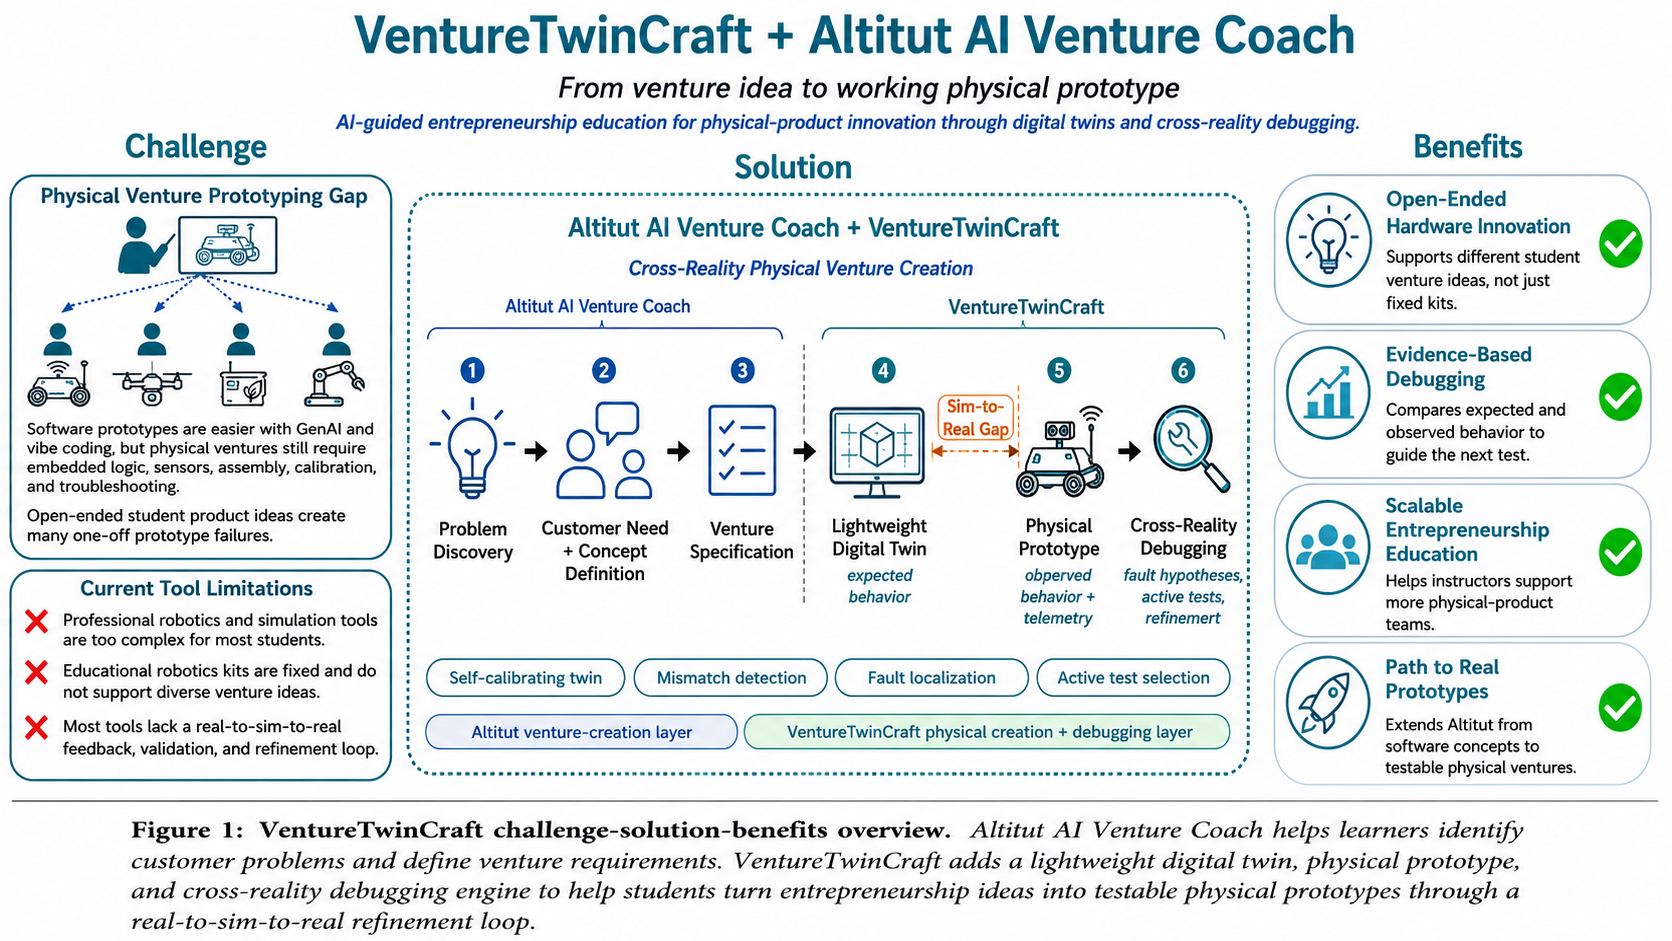
\includegraphics[width=\linewidth]{images/Idea2_GPT.png}
    \caption{Picture from GPT}
    \label{fig:placeholder}
\end{figure}

\section{1. Technology Innovation}

The proposed Phase I innovation is an uncertainty-aware cross-reality diagnostic architecture that continuously aligns a lightweight digital twin with a low-cost physical prototype and actively selects diagnostic experiments to identify the causes of sim-to-real discrepancies.

Generative AI and AI-assisted coding tools can suggest components, generate embedded code, and provide assembly instructions. However, once a real prototype is assembled, these systems have limited ability to determine why the physical device does not behave as predicted. A failure may result from inaccurate model parameters, component variation, sensor noise, wiring or configuration errors, firmware defects, insufficient power, mechanical resistance, or environmental conditions. Different causes may produce similar observable symptoms, and general-purpose AI tools typically return generic troubleshooting lists without maintaining a model of expected system behavior or selecting the next test based on uncertainty.

VentureTwinCraft will investigate a cross-reality reasoning engine that maintains two continuously linked representations: a lightweight digital twin of expected device behavior and a physical-state representation derived from telemetry, controller logs, actuator response, timing data, and selected user observations.

The proposed architecture will:

estimate and update uncertain digital-twin parameters from sparse physical-device observations;
detect statistically and functionally meaningful differences between expected and observed behavior;
generate competing hypotheses spanning model, hardware, firmware, configuration, and environmental causes;
maintain calibrated uncertainty over those hypotheses;
select the next diagnostic experiment expected to provide the greatest information gain; and
update both the digital twin and fault model after each test.

The foundational innovation is not the hardware kit, chatbot, or digital twin alone. It is the integration of online system identification, uncertainty-aware fault reasoning, and active diagnostic test selection for heterogeneous, novice-built physical prototypes with incomplete and noisy observations.

Professional digital-twin and robotics platforms are designed for expert users and controlled systems with detailed models. Educational robotics systems generally use fixed kits and predefined projects. General-purpose LLMs lack persistent physical-state models and cannot reliably distinguish among competing physical fault causes.

If successful, the research would create a technical pathway for students and non-engineers to diagnose and refine open-ended physical-product prototypes without requiring continuous one-on-one intervention from an embedded-systems expert.

\section{2. Technical Objectives and Challenges}

The Phase I research objective is to test the hypothesis that an uncertainty-aware active-diagnosis method using a continuously calibrated lightweight digital twin can identify the root causes of physical-prototype failures with greater accuracy and fewer diagnostic tests than general-purpose LLM assistance, static troubleshooting workflows, or fault classifiers without an adaptive digital twin.

Phase I will use a bounded modular hardware environment consisting of one microcontroller family, a validated set of low-voltage sensors and actuators, standardized telemetry, and a small number of tabletop device classes.

\subsection{Objective 1: Online calibration of lightweight digital twins.}
The system will estimate device-specific parameters such as sensor bias, actuator response curves, latency, noise, threshold behavior, and load-dependent performance from limited physical observations. The main challenge is parameter identifiability: different combinations of inaccurate model assumptions and physical faults may produce similar behavior. The research will evaluate sequential system-identification methods that represent estimated parameters as probability distributions rather than fixed values.

\subsection{Objective 2: Cross-reality mismatch detection and fault localization.}
The system will compare predicted and observed behavior and distinguish among model error, component variation, wiring or configuration faults, firmware logic defects, and environmental or mechanical effects. The challenge is partial observability and fault ambiguity. Multiple causes may generate similar sensor and actuator traces, and more than one fault may occur simultaneously. The proposed approach will use probabilistic fault hypotheses linked to digital-twin predictions and diagnostic evidence.

\subsection{Objective 3: Active diagnostic experiment selection.}
The system will select the next test expected to reduce uncertainty most effectively. Candidate tests may include running an actuator without load, isolating a sensor, applying a controlled input, executing a calibration routine, or modifying a firmware configuration. The technical challenge is selecting tests that are informative, feasible for a novice, and safe for the supported hardware.

Phase I evaluation will use repeatable prototype tasks with intentionally introduced model, hardware, firmware, calibration, and environmental faults. Baselines will include static troubleshooting guides, general-purpose LLM recommendations based on logs and user descriptions, and a supervised fault classifier without active test selection.

Measures will include digital-twin parameter-estimation error, mismatch-detection accuracy, fault-localization accuracy, calibration of diagnostic uncertainty, number of tests required to identify a root cause, successful repair rate, time to a functioning prototype, and frequency of incorrect or unsafe recommendations.

The hypothesis will be falsified if the proposed method does not significantly improve diagnosis efficiency and accuracy across the bounded hardware classes or if its uncertainty estimates fail to reliably identify cases requiring expert intervention.

\section{3. Market Opportunity}

The initial customers are high-school CTE, engineering, and robotics programs; community-college makerspaces; university entrepreneurship centers; after-school maker programs; and workforce technical-training laboratories.

These organizations increasingly want learners to develop open-ended physical products rather than assemble identical predefined kits. However, open-ended projects generate many unique failures involving sensors, wiring, embedded software, calibration, power, and mechanical behavior. Instructors and technical staff must diagnose each project individually, limiting the number and diversity of ventures that programs can support.

Existing alternatives include fixed robotics kits, video tutorials, general-purpose AI assistants, circuit-design tools, and professional simulation or digital-twin platforms. Fixed kits reduce troubleshooting complexity but restrict student creativity. Generic AI tools may provide plausible advice but do not compare predicted and observed system behavior or systematically identify the most informative next test. Professional platforms require engineering expertise and detailed system models.

VentureTwinCraft would provide a cross-reality diagnostic layer for supported modular hardware, enabling programs to retain open-ended project choice while reducing repetitive expert troubleshooting.

The first commercial offering could combine institutional software licensing, a supported component ecosystem, student project interfaces, and an instructor dashboard. Integration with Altitut AI Venture Coach would connect customer discovery and venture definition to physical prototyping, testing, refinement, and pitching.

The near-term value proposition is to help one instructor support more physical-product teams and increase the proportion of student ideas that reach a functioning, testable prototype.

\section{4. Company and Team}

Altitut LLC develops AI-supported entrepreneurship education tools that guide learners through problem discovery, customer interviews, concept development, user testing, business-model refinement, and venture pitching. The company’s platform, educator relationships, and experience supporting learner-owned projects provide the entrepreneurship and commercialization layer for VentureTwinCraft.

The proposed PI would lead product and research definition, educational use-case development, customer discovery, project coordination, and integration with the Altitut AI Venture Coach. Altitut’s software and AI team would support data infrastructure, model integration, workflow design, and student and instructor interfaces.

Altitut’s principal contribution is its understanding of how learners move from an identified customer problem to a venture concept and testable value proposition. VentureTwinCraft would extend that workflow into physical-product creation by providing digital-twin calibration and cross-reality diagnosis.

The current team has material gaps in embedded systems, control systems, digital twins, system identification, probabilistic fault diagnosis, and hardware safety. These gaps must be addressed before submission of a full proposal. Altitut will recruit or formally engage an embedded-systems or controls technical lead with relevant research and prototype-development experience. Additional advisors or collaborators will support active diagnosis, robotics, and hardware validation.

Phase I will be limited to a bounded low-voltage modular hardware ecosystem so that the proposed technical questions can be investigated safely and reproducibly. Educational and makerspace partners will help define representative prototype tasks and validate the commercial pain point.


1. With the vibe coding (which year start), it improve the efficiy and 受众 for software development. Efficincy: the vibe coding improve the idea generation - plan -testing -debug - lauch develop loop from months to weeks. 受众：vibe coding (Gen AI) even if users has limited knowledge in softare development or engineer, as long as they have an idea, they can create some product. 2. However, the current hardware design still not match this fast develop pace and need improve.. For example, the current robotics company Mmmoten, Pyrellis, VEX robot still needs months (usually > 1year) to finish the whole develop and prototype validation. 3. current altitut llc's preliminary work, an entrepreneur AI assistanet platform validate the market need in entrepreneurship and success support students in build software, but still gaps in hardware because of the long develope loop and missing of validation (simulation), hardware can't scale/acceleration. Especially in venture project, different students share different ideas and have different hardware requirments. 4. We propose a "vibe coding" method for hardware for this phase I. software and math modeling simulation/validation before the hardware assemblely. step1: basing on current Gen AI/ LLM/ Gemma, and users input (venture project idea), Gen AI generate the corresponding datasheet (how to assembly and unserdatnd how they interact with each other, how electronic signal should be simulation, how noisy signal looks like) + physical kits (AI suggest what needed to build up the things, like wifi). Step 2: in the simulation step, we will provide a software, so the students can pre-validate their ideas/thoughs before real life assemblly, which we will introduce all kinds of math modeling build up , so the simulation will include math/model simulation + calibration + debugging + education (reasoning/explaination) in prototyes for hardward/3D priting. In future phase, we will do the real-sim-real through VR tech to dignosize the real hardware assembly issue and use AI + build in step2's math reasoning model to give feedback. The tech issue is : need build correspodning and consistent math model on simulation platform basing on different hardware requirments, for example, 3D printer, need math model to varify the physical structure in steability or any others; electrical engineer board, need math model 傅里叶变化，to analysis real world nosiy signal to keep resilliance in the physical-aware machine learning; for some 人脸识别项目，need test build machine learning model. Our simulation software targets to provide an real workspace simulation to test debug and reason explaining with math things 下面是我和我老板meeting 的scratch “This proposal work ->VentureMath Altitut -> prelimenary work prelimenary work Altitut-> software SW focus venture creation problems is that Hardware cannot scale Math: simulation physics-aware machine learning EE modeling (nosiy signal) sw creation, hw acceleration. in-order to do hw, need domain knolwge/pre-knowledge of pyhsics. Foundmental math. EE modeling (Key personal) EE design: datasheets -> step1: put into Gemma (Altitut) current LLM, get basic requirments wifi, what components 1,2,3,4,... we need reading the data sheet and understanding how they interaction with each other, need simulation (wifi) -> step2: Mmmoten/Pyrellis/VEX robot, problem -> prototyping, newest design requirment need fuuncation: wifi, (need adapt to coding very fast), stimulate the process LLM brainstorming, datasheets (how electronic signoal), testing, debuging, remagining datasheets + breakout boards Datasheets + Breakout boards -> reference designs (like raseberry pi) prelimineary work on SW, HW two gap: firmware + software + hardware Math element in simulation + catlization + debugging + education (in prototyes) math into 3D printing gap, current HW develop too slow letter of support, if she wants to come”


A verified project-to-mathematics translation architecture that extracts quantitative structures from evolving student ventures, generates multiple mathematically equivalent representations, and automatically verifies their correctness, evidentiary grounding, and instructional suitability.

\section{VentureTwinCraft Overview}

Generative AI and “vibe coding” have substantially lowered the barrier to software prototyping in entrepreneurship education. Students can now translate a product idea into a website, application, or interactive software demonstration with limited programming experience. However, no comparable end-to-end pathway exists for physical-product ventures. Students who want to develop a sensor-based device, interactive object, or simple robot must still bridge multiple technical domains, including requirements engineering, component selection, embedded programming, physical assembly, calibration, simulation, and troubleshooting.

Existing professional robotics and physics-simulation platforms are primarily designed for trained engineers and researchers and require substantial technical expertise. AI-assisted electronic-design tools can support schematic or component-level design, while educational robotics platforms generally rely on fixed kits, predefined projects, and standardized assembly sequences. These approaches do not adequately support students developing different physical products in response to independently identified customer problems. More importantly, they typically lack an integrated feedback loop that continuously compares a digital model with the student’s physical prototype, identifies the source of sim-to-real discrepancies, and guides iterative testing and refinement.

\textbf{VentureTwinCraft} is a proposed AI-guided physical venture-creation environment integrated with the \textbf{Altitut AI Venture Coach}. Altitut would provide the entrepreneurship-development layer, guiding learners through problem discovery, customer interviews, requirements definition, value-proposition development, user testing, business-model refinement, and venture pitching. VentureTwinCraft would add a physical-product development layer that helps learners translate validated customer needs into bounded, testable hardware prototypes.

The candidate foundational innovation is an \textbf{uncertainty-aware cross-reality reasoning and debugging engine}. The engine would maintain a lightweight digital twin representing the expected behavior of a proposed physical product and continuously compare that model with observations from the real prototype. These observations may include sensor telemetry, controller and firmware logs, timing data, actuator responses, user-provided test results, and, where appropriate, visual observations.

Rather than returning a generic troubleshooting checklist, the proposed system would:

\begin{itemize}
    \item detect statistically and functionally meaningful discrepancies between expected and observed behavior;
    \item generate competing hypotheses related to model error, component variation, wiring or configuration faults, firmware defects, calibration problems, and environmental effects;
    \item quantify uncertainty across those hypotheses;
    \item select the next diagnostic experiment expected to provide the greatest information gain;
    \item update both the digital twin and the fault hypotheses based on the result; and
    \item guide the learner through evidence-based refinement of the physical prototype.
\end{itemize}


The proposed R\&D draws inspiration from recent real-to-sim-to-real research, but applies the paradigm to a different technical and commercial problem: enabling novice creators to develop, diagnose, and refine heterogeneous physical-product prototypes. The objective is not to reproduce a professional robotics platform or merely add an AI assistant to a hardware kit. The research question is whether sparse, noisy observations from low-cost modular hardware can be used to construct and continuously calibrate an actionable digital twin that supports reliable cross-reality diagnosis.

A Phase I project would initially be limited to one microcontroller family, a validated library of low-voltage sensors and actuators, and a small number of tabletop product classes. The research would evaluate three foundational capabilities:
\begin{itemize}
    \item generation of structured venture and engineering requirements from customer-validated product concepts;
    \item online calibration of lightweight digital twins using sparse and noisy physical-device observations; and
    \item uncertainty-aware active diagnosis that identifies root causes with fewer tests and less expert intervention than general-purpose LLM assistance or static troubleshooting workflows.
\end{itemize}

Technical performance would be evaluated using digital-twin parameter error, mismatch-detection accuracy, fault-localization accuracy, number of tests required to identify a root cause, successful prototype-repair rate, time to a functioning prototype, and frequency of incorrect or unsafe recommendations.

The initial market would include secondary and postsecondary entrepreneurship programs, CTE and robotics programs, makerspaces, incubators, and workforce-development organizations. VentureTwinCraft would extend Altitut from helping students determine \textbf{what to create, for whom, and why} to helping them understand \textbf{how a physical prototype should behave, why the real implementation differs, and what evidence-based action should be taken next}.


\newpage

\section{1. VentureMath Overview}
Mathematics is foundational to entrepreneurship, financial decision-making, engineering, computing, and the physical sciences. Entrepreneurs rely on percentages, pricing, revenue, cost, profit, forecasting, probability, statistics, and optimization. Product teams use statistical analysis and A/B testing. Electrical engineers apply Fourier analysis and complex analysis, computer scientists use graph theory and number theory, and physicists rely on mathematical modeling, differential equations, and advanced geometry.

However, many K–12 students experience mathematics as abstract, disconnected from their interests, and difficult to apply outside the classroom. Students may learn formulas and procedures without understanding how mathematical relationships influence decisions in projects, businesses, technologies, and everyday life.

\section{2. Market Gap}

Existing entrepreneurship education programs, including mentor-supported and project-based programs, help students develop venture ideas and basic business skills. However, these programs often depend heavily on teachers, volunteers, or industry mentors and generally do not provide individualized instruction in the mathematical concepts required to develop and evaluate each student’s venture.

Conversely, existing mathematics learning platforms primarily deliver predefined lessons, practice problems, or adaptive exercises. Although these platforms may personalize difficulty, they typically do not connect mathematics to a learner-owned venture, product idea, creative project, or authentic decision-making context.

As a result, a market gap exists between:
\begin{itemize}
    \item entrepreneurship platforms that provide authentic projects but limited personalized mathematics support; and
    \item mathematics platforms that teach concepts but lack meaningful, student-owned applications.
\end{itemize}

\section{3. Proposed Solution}

VentureMath is an AI-supported mathematics and financial-literacy environment that transforms each student’s entrepreneurial or creative project into a personalized, interactive mathematics learning experience.

Students begin with an idea they care about, such as a small business, digital product, game, community service, content channel, or physical invention. VentureMath identifies the mathematical concepts embedded in that project and helps the learner apply them to authentic decisions involving:
\begin{itemize}
    \item cost, price, revenue, and profit;
\item budgeting and personal finance;
\item percentages, ratios, and proportional reasoning;
\item market surveys and statistical analysis;
\item probability and risk;
\item growth functions and forecasting;
\item break-even analysis;
\item customer experiments and A/B testing;
\item and resource-allocation decisions.
\end{itemize}


Rather than presenting mathematics only through formal notation, VentureMath generates multiple interest-connected representations of the same mathematical structure. For example, a function may be represented through a business growth model, an interactive graph, physical motion, a game mechanic, or changes in musical pitch and rhythm.

The goal is not to replace formal mathematics with entertainment. The system helps learners move from a familiar project or representation to an interactive model and ultimately to rigorous mathematical notation and transferable understanding.

\section{4. Core Deep-Technology Innovation}

The proposed deep-technology innovation is a verified project-to-mathematics translation architecture that converts incomplete, evolving student project information into mathematically valid and instructionally appropriate learning models.

Unlike a general-purpose generative AI system that produces plausible explanations or word problems, VentureMath would combine generative AI with structured mathematical representations, executable models, domain constraints, and automated verification.

The proposed architecture would perform four technically challenging functions:

\subsubsection{A. Project-to-Mathematical-Model Extraction}

The system would identify variables, quantitative relationships, constraints, assumptions, units, uncertainty, and available evidence from unstructured student artifacts such as venture descriptions, budgets, surveys, interview findings, pricing ideas, and project records.

For example, the system would distinguish between:

\begin{itemize}
    \item verified material costs and estimated costs;
\item observed customer demand and unsupported demand assumptions;
\item fixed costs and variable costs;
\item revenue, cash flow, and profit;
\item and mathematical relationships that are appropriate for the student’s grade level.
\end{itemize}

\subsection{B. Structure-Preserving Multimodal Translation}

The system would translate one mathematical model into multiple visual, contextual, auditory, and interactive representations while preserving the same underlying mathematical relationships.

For example, when representing a function through music, animation, a business scenario, and a graph, the system must maintain consistent mappings among variables, parameters, rates of change, boundary conditions, and outputs.

This differs from conventional generative AI, which may generate attractive examples without guaranteeing that the representations are mathematically equivalent.

\subsection{C. Automated Mathematical and Evidentiary Verification}

A verification layer would test whether AI-generated models, simulations, examples, and explanations are consistent with:
\begin{itemize}
    \item the source mathematical relationship;
\item units and dimensional constraints;
\item arithmetic and functional behavior;
\item the student’s actual project evidence;
\item grade-appropriate standards;
\item and the assumptions stated by the system.
\end{itemize}


When the available project information is insufficient, the system would request clarification or explicitly identify uncertainty rather than generate an unsupported conclusion.

\subsection{D. Adaptive Reasoning and Feedback}

VentureMath would evaluate how students make decisions within interactive project scenarios, not only whether they enter the correct numerical answer.

The system would use student predictions, explanations, parameter changes, and responses to counterexamples to identify possible misconceptions and select the next representation, question, or simulation that can best clarify the learner’s reasoning.

Teachers would remain in the loop through a dashboard showing the mathematical concepts used, project evidence, student reasoning, detected uncertainties, and areas requiring instructor review.

\section{5.Expected Value}

VentureMath would help students experience mathematics as a practical tool for creating, evaluating, and improving ideas they personally value.

For students, the platform could increase relevance, mathematical confidence, financial literacy, and the ability to transfer mathematical reasoning across different contexts.

For teachers, it could reduce the time required to create individualized project-based mathematics activities and provide greater visibility into each learner’s reasoning.

For schools, VentureMath could connect mathematics, financial literacy, entrepreneurship, career readiness, and project-based learning within a unified instructional environment.

For Altitut, the technology would extend the company’s existing entrepreneurship workflows, student project data, and educator relationships while introducing a differentiated mathematical modeling, verification, and adaptive-learning capability.

VentureMath overview.  Math Education  is tough becuase most of the math concept is too abstract for students to understand. But Math is import, because it’s the foundation of business (econmy, income, revenue calculation, finance), Product (statistics, A/B testing), electronic engineer (frontier analysis, complex analysis), computer science (graph, number theory), physics (topology analysis). There are still gaps in the current market, eithr JA (Junior Achievement), BizWorld/VentureLab.org teach students with vonlunteered mentor (for example, bank manager), lack one-on-one personalized math concept teaching and feedback. Or math concept Education platform, which lacking the real venture project to improve student’s willingness to learn math. Real time VentureMath targets at using the students’ most familar language (Venture idea, the entrepreneurship education and topic students interested in most, since they need to create their own idea) to help students:
掌握 neccesary math concepts for their venturn, finacial related things and business model? revenue, and so on
帮助他们理解 abstract math model in the language they like, for example, understand function in the sound of music (with AI’s help and need double verification, the AI generated other domains way to explain the math concept is correct, not just the Gen AI, this should be our key tech and deep tech) 

ventureMath fixed this gaps by use multimodal (depends on the students’ most interested project)in entrepreneurship product (real venteneur real life needed knowledge) to help students understand abstract math concept easly, interestingly and improve their interet


################Idea 2##################
VentureTwinCraft overview.  Entrepreneurship Education is currently relative easy for software prototype with the help of vibe coding and gen AI but still empty for hardware/physical product generated.  Currently gap is either NVIDIA and Physical Intelligence targets for profesionals, platform too complex for students or  Flux.ai, Vinci4D  lacking sim-to-real, cross-validation-feedback-refine loop is missing. EdTech like AI+Scratch/lego targets for LLM/AI courses no customized design, fixed kit only which is not supported for different entrepreneurship idea design. We will explore real-to-sim-to-real MIT SCAIL RialTo system tech to see if the research project can build in to the Altitut and support digital twin + physical prototye, cross-reality debugging engine to help make students entrepreneurship idea transfer to a real prototye not just a software concept
